% !TeX spellcheck = ru_RU-Russian
\documentclass[utf8,12pt]{jetp}
%\twocolumn

\def\baselinestratch{1.5}

\DeclareMathOperator{\arcsh}{arcsh}
\DeclareMathOperator{\arcch}{arcch}
\DeclareMathOperator{\Det}{Det}
\DeclareMathOperator{\Cl}{Cl}
\DeclareMathOperator{\Li}{Li}
\DeclareMathOperator{\im}{Im}

\DeclareUnicodeCharacter{2212}{\textendash}

\begin{document}

\title{Обобщенная модель Изинга на квадратной решетке}
	
\setaffiliation1{Российский федеральный ядерный центр --- ВНИИТФ им. академика Е. И. Забабахина, 456770, Снежинск, Челябинская обл., Россия} %
\setaffiliation2{Институт физики металлов им. М. Н. Михеева  Уральского отделения Российской академии наук \\ 620108, Екатеринбург, Россия}
	
\setauthor{Е.~С.}{Цуварев}{12}
\email{eguny@mail.ru}
	
\setauthor{Ф.~А.}{Кассан-Оглы}{2}
\email{felix.kassan-ogly@imp.uran.ru}

	
\rtitle{Обобщенная модель Изинга на квадратной решетке}
\rauthor{Е.~С.~Цуварев, Ф.~А.~Кассан-Оглы}
	
	
\abstract{Впервые выведено точное аналитическое решение для свободной энергии Гельмгольца в обобщенной модели Изинга на квадратной решетке комбинаторным методом Вдовиченко--Фейнмана. Исследованы термодинамические, магнитные и фрустрационные свойства обобщенной модели Изинга на квадратной решетке с двумя трансляциями в горизонтальном и вертикальном направлениях. Установлены новые особенности, возникающие в обобщенной модели Изинга.}
	
\maketitle

\section{Введение}

В текущем календарном году исполняется ровно сто лет со времени опубликования исходной статьи по классической модели Изинга на линейной регулярной одноатомной цепочке спинов с двумя состояниями в присутствии внешнего магнитного поля и с обменным взаимодействием только между ближайшими соседями Эрнстом Изингом в журнале Zeitschrift für Physik под названием Beitrag zur Theorie des Ferromagnetismus~\cite{ising1925}. Изинг произвел детальный точный расчет свободной энергии Гельмгольца и продемонстрировал, что при обозначенных условиях не наблюдается никакого фазового перехода ни при какой конечной температуре. На основе полученных результатов он сделал заключение, что в рассматриваемой модели не может быть фазового перехода при любых размерностях.

Однако в 1936 году Рудольф Пайерлс опубликовал статью~\cite{peierls1936}, в которой вопреки утверждению Изинга, он доказал, что модель Изинга должна испытывать переход в 2D и 3D случаях. В 1941 году Крамерс и Ваннье при сопоставлении низкотемпературного и высокотемпературного разложения статистической суммы и с помощью изобретенного ими дуального превращения вычислили критическую температуру фазового перехода в модели Изинга на квадратной решетке с обменным взаимодействием между ближайшими соседями по горизонтальному и вертикальному направлению~\cite{kramers_wannier1, kramers_wannier2}.

Впоследствии в 1944 году~\cite{onsager1941} Онзагер, используя метод трансфер-матрицы Крамерса-Ваннье весьма сложным методом, основанным на алгебрах Ли, получил точное аналитическое решение для свободной энергии Гельмгольца в модели Изинга на квадратной решетке. Эта работа открыла новую эпоху и фактически определила границу размежевания между предыдущими наивными, весьма упрощенными теориями типа молекулярного поля и современной эрой исследования критических явлений в статистической физике с сопутствующими особенностями поведения термодинамических величин. 

Труднопреодолимость весьма сложного оригинального метода Онзагера, а, главное, выдающийся результат Онзагера побудил многих высококлассных исследователей, как физиков, так и математиков, к поискам самых разнообразных направлений обобщений по разработке более простых и эффективных методов получения точных решений с одной стороны, а с другой стороны, к расширению объектов и задач исследований. Точное аналитическое решение для свободной энергии Гельмгольца в модели Изинга на квадратной решетке было успешно переполучено в разнообразных комбинаторных подходах, развитых, в частности, Кацем и Вардом~\cite{kac1952}, Поттсом и Вардом~\cite{potts1955}, Херстом и Грином~\cite{hurst1960}, Вдовиченко~\cite{vdovichenko1964, vdovichenko1965}, Фейнманом~\cite{feynman1972}, а в более поздних теориях, основанных на грассмановых переменных: Самуэлем~\cite{samuel1980}, Плечко~\cite{plechko1985}, а также с использованием алгебры Клиффорда-Дирака Вергелесом~\cite{vergeles2009}.

К настоящему времени, количество научных статей по модели Изинга исчисляется тысячами и тысячами, и продолжает только увеличиваться, не обнаруживая спада активности. Однако следует отметить, что, несмотря на огромные затраченные усилия, направленные на поиски точных решений для свободной энергии в ряде случаев оказались не решенными до сих пор. Во-первых, это невозможность обобщения на 3D объекты. Во-вторых, отсутствие решений во внешнем магнитном поле ни на одной из 2D решеток. В-третьих, точно установлено, что решениям поддаются не все 2D решетки, а только лишь планарные, то есть те, в которых отсутствуют пересечения между обменными взаимодействиями. В-четвертых, модель Изинга при обобщении на спины с числом состояний более двух также не поддается точному решению. 

Ввиду указанных непреодолимых препятствий на пути более углубленных исследований, интересы исследователей постепенно переключались на применение модели Изинга к более широким объектам, в частности, 2D планарным решеткам: к классу одиннадцати Архимедовых и классу дуальных Архимедовым восьми решеток Лавэ; подробное изложение свойств решеток этих классов и строгое доказательство их уникальности изложено в книге Грюнбаума и Шефарда~\cite{grunbaum1987}. 

К настоящему времени точные выводы свободной энергии Гельмгольца получены на многих Архимедовых  решетках, в том числе: на квадратной решетке Онзагером~\cite{onsager1941}, на треугольной решетке Ваннье~\cite{wannier1950}, на гексагональной решетке Гутаппелем~\cite{houtapell1950}, на решетке кагоме Кано и Найем~\cite{kano_naya1953}, на решетке баунс (ruby) Лином и Ма~\cite{lin1983}, на решетке кросс (решетка 4-6-12) Лином и Хуангом~\cite{lin1985}. 

Точные решения свободной энергии Гельмгольца в модели Изинга получены и на некоторых решетках Лавэ (которые являются дуальными Архимедовым  решеткам); среди них: Ваксом, Ларкиным и Овчинниковым на решетке Union Jack~\cite{vaks1965}, Урюмовым на решетке Cairo pentagonal~\cite{urumov2002}, Хольцером на Dice решетке~\cite{holzer1990}.

Существуют также точные выводы свободной энергии Гельмгольца на ряде решеток, не входящих ни в класс Архимедовых, ни в класс Лавэ, в частности, Лином и Вангом на одном типе решетки 4-6~\cite{lin1988}, Оитмаа и Кеппертом на другом типе решетки 4-6~\cite{oitmaa2002}, Стречкой и Кановой на решетке bow-tie~\cite{strecka2008}, Чао, Лии и Лином на решетке 3-6~\cite{chao1990}, а также Ло, Яо и Карлсоном на решетке TKL (triangular kagome lattice)~\cite{loh2008}.

Поскольку точному решению поддаются только планарные решетки, а даже учет взаимодействия между спинами на вторых соседях не отвечает условию планарности, то интерес исследователей переключился на новое направление, а именно, возникли множественные попытки решить задачу в случае только взаимодействий между ближайшими соседями, но разных между разными соседними спинами. Фактически это означает переход на более высокий уровень — исследование решеток с трансляциями на два периода решетки по всем направлениям. Строго говоря, на всех указанных выше решетках такая задача решается как бы компромиссным образом — число учитываемых взаимодействий больше, чем с трансляциями на один период решетки, но меньше, чем на два периода. 

В качестве примера рассмотрим историю исследования решетки Union Jack. Первоначально, Ваксом, Ларкиным и Овчинниковым~\cite{vaks1965} свободная энергия Гельмгольца выведена точно, при учете двух взаимодействий (исходная решетка с трансляциями на один период решетки по двум направлениям), затем Чикью и Сузуки~\cite{chikyu1987} сосчитали свободную энергию Гельмгольца с тремя обменными взаимодействиями, Морита~\cite{morita1986} обобщил задачу на четыре взаимодействия, и позднее Ву и Лином~\cite{wu1987} задача решена точно с учетом шести взаимодействий. И, тем не менее, окончательного решения не найдено, поскольку в решетке Union Jack с трансляциями на два периода решетки число обменных взаимодействий равно восьми. В итоге получается, что задача с трансляциями на два периода решетки до конца не решена ни на одной из решеток, кроме одной, а именно, на квадратной решетке, причем без какого либо вывода и исследования свойств полученного выражения, (см., например,~\cite{syozi1972, utiyama1951}).

Целями настоящей работы является вывод точного аналитического выражения для свободной энергии Гельмгольца в модели Изинга на квадратной решетке с трансляционной инвариантностью на два периода решетки в горизонтальном и вертикальном направлениях с использованием наиболее удобного и эффективного метода Вдовиченко-Фейнмана, а также исследование физических свойств полученного решения при произвольном варьировании величин и знаков всех четырех обменных взаимодействий.

\section{Вычисление свободной энергии комбинаторным методом}

История комбинаторного метода начинается с важной работы Каца и Уорда~\cite{kac1952}. В попытках получить более интуитивное решение двумерной модели Изинга, авторы предположили, что нахождение статсуммы можно свести к некоторой комбинаторной задаче. В этой статье авторы рассмотрели разложение статсуммы в форме Ван дер Вардена~\cite{warden1941} как сумму по определенным множествам замкнутых циклов (или путей) на решетке. Основываясь на топологической гипотезе, авторы установили соответствие между суммой по замкнутым циклам и определителем, построенного по некоторым правилам. В результате, авторы переполучили точное решение Онзагера. Работа вводит графовое представление модели, где ребра графа соответствуют взаимодействиям между спинами. Комбинаторный подсчет циклов на этом графе становится ключевым инструментом. Именно эта работа дала совершенно новый взгляд на проблему, однако решение все еще оставалось технически сложным и неполным. Тем не менее, статья Каца и Уорда заложила фундамент для дальнейшего развития комбинаторных методов, показав важность графовых структур и циклов. 

Статья Поттса и Уорда 1955 года~\cite{potts1955} стала значительным расширением и обобщением идей Каца и Уорда. Если Кац и Уорд сосредоточились на комбинаторном решении двумерной модели Изинга, то Поттс и Уорд распространили эти методы на получение корреляционной функции. Это существенно расширило область применения комбинаторных методов в статистической механике и углубило понимание фазовых переходов и критических явлений. В результате авторы практически переполучили результат Кауфман~\cite{kaufman1949} для парной корреляционной функции на квадратной решетке.

Затем Херст и Грин~\cite{hurst1960} значительно упростили расчет, предложенный Кацем и Уордом. Авторы ввели метод подсчета циклов на решетке с использованием алгебры пфаффианов. Их подход позволял свести задачу к вычислению определителей и матриц, связанных с графом решетки. Они связали статсумму с определителем некоторого оператора, что открыло путь к более чистому и элегантному решению. Работа Херста и Грина фактически является мостом между чисто комбинаторным подходом и алгебраическими методами решения.
 
Впоследствии, Вдовиченко~\cite{vdovichenko1964, vdovichenko1965} и Фейнман~\cite{feynman1972} доработали идею комбинаторного метода. Вдовиченко разработала детальное решение двумерной модели Изинга, используя методы теории графов и определителей, что позволило получить точное выражение для статсуммы. Фейнман, в свою очередь, выдвинул догадку, о том что, замкнутые циклы на решетке по своей сути являются марковскими цепями. Поэтому, поиск всех возможных замкнутых не пересекающихся циклов на решетке различной длины сведется к задаче о случайных блужданиях. Их идеи, в конце концов, позволили получить точное решение двумерной модели Изинга наиболее простым способом.

В работе~\cite{generalizedIsing2021} была упомянута квадратная решетка с обобщением на две трансляции в горизонтальном и вертикальном направлениях, предложенное Сиози (рис.~\ref{gen}). В своих работах Сиози \cite{syozi1972} предложил формулу для расчета свободной энергии Гельмгольца (но без доказательства). В данной статье будет получено точное аналитическое решение обобщенной модели Изинга на квадратной решетке с помощью комбинаторного метода Вдовиченко--Фейнмана.

\begin{figure}[h]
	\center{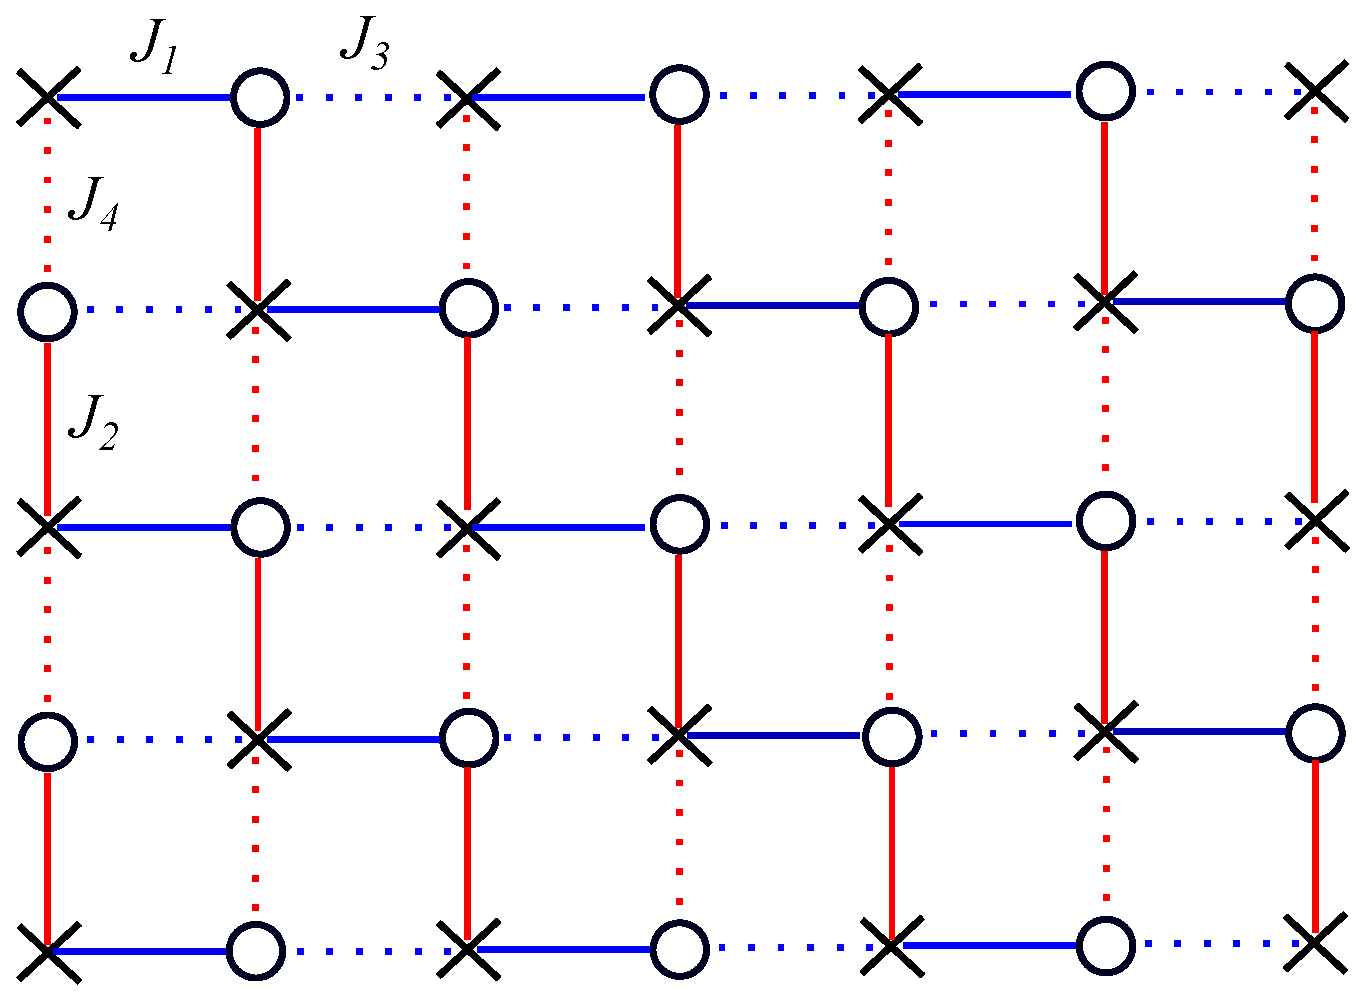
\includegraphics[width=0.6\linewidth]{Pictures/gen.eps}}
	\caption{Обобщенная квадратная решетка}
	\label{gen}
\end{figure}

Статсумму приведенной квадратной решетки (рис.~\ref{gen}) можно представить следующим образом 
\begin{equation}
Z_{N} = \sum_{\{\sigma\}} \exp{\bigg[ K_1 \sum_{\substack{i = 1,3,\dots \\ j = 2,4,\dots}} \sigma_i \sigma_j + K_2 \sum_{\substack{i = 2,4,\dots \\ k = 3,5,\dots}} \sigma_i \sigma_k + K_3 \sum_{\substack{i = 2,4,\dots \\ j = 3,5,\dots}} \sigma_i \sigma_j + K_4 \sum_{\substack{i = 1,3,\dots \\ k = 2,4,\dots}} \sigma_i \sigma_k\bigg]},
\end{equation}
где первая и третья суммы идут по половинам спинов в горизонтальном направлении,  а вторая и четвертая суммы идут по половинам спинов в вертикальном направлении, так что
\begin{equation*}
K_1 = \frac{J_1}{T}; \;\;\;\;\;\; K_2 = \frac{J_2}{T};\;\;\;\;\;\; K_3 = \frac{J_3}{T};\;\;\;\;\;\;K_4 = \frac{J_4}{T}.
\end{equation*}

Перепишем статсумму в виде
\begin{align}
&Z_{N} = (\ch K_1 \ch K_2 \ch K_3 \ch K_4)^N S, \nonumber \\
&S = \sum_{\{\sigma\}} \prod_{\substack{i = 1,3,\dots \\ j = 2,4,\dots}} (1 + v \sigma_i \sigma_j) \prod_{\substack{i = 2,4,\dots \\ k = 3,5,\dots}} (1 + u \sigma_i \sigma_k) \times \nonumber\\&\;\;\;\;\;\;\;\;\; \times \prod_{\substack{i = 2,4,\dots \\ j = 3,5,\dots}} (1 + w \sigma_i \sigma_j) \prod_{\substack{i = 1,3,\dots \\ k = 2,4,\dots}} (1 + t \sigma_i \sigma_k).
\label{z} 
\end{align}

Здесь $v = \th K_1$, $u = \th K_2$, $w = \th K_3$, $t = \th K_4$, а $N = L^2$ --- число спинов в решетке. Величина $S$ является полиномом от $v$, $u$, $w$ и $t$, в котором коэффициент $g_{nmlk}$ при $v^n u^m w^l t^k$ равен количеству способов построения замкнутых многоугольников, при которых общее количество горизонтальных связей равно $n+l$, а общее количество вертикальных связей равно $m+k$.

В статье Вдовиченко~\cite{vdovichenko1965} было показано, что для модели Изинга на обычной квадратной решетке величина $g_{nmlk}$ может быть представлена в виде суммы по замкнутым циклам, причем каждый цикл берется с множителем $(-1)^s$, где $s$ --- количество самопересечений замкнутого многоугольника. Вариант с обобщенной квадратной решеткой нисколько не отличается от обычного, за исключением того, что на обобщенной квадратной решетке встречаются два вида узлов (рисунок \ref{point}) (см. статьи~\cite{vaks1965, chikyu1987}). У узла, помеченного крестом (рисунок \ref{point}а), связь между соседним верхним узлом с обменным взаимодействием $J_2$, между соседним нижним узлом --- $J_4$, между соседним левым узлом --- $J_3$, между соседним правым узлом --- $J_1$. У узла, обозначенного кружком (рисунок \ref{point}б), наоборот: связь между соседним верхним узлом с обменным взаимодействием $J_4$, между соседним нижним узлом --- $J_2$, между соседним левым узлом --- $J_1$, между соседним правым узлом --- $J_3$. 

\begin{figure}[h]
	\begin{minipage}[h]{0.4\linewidth}
		\center{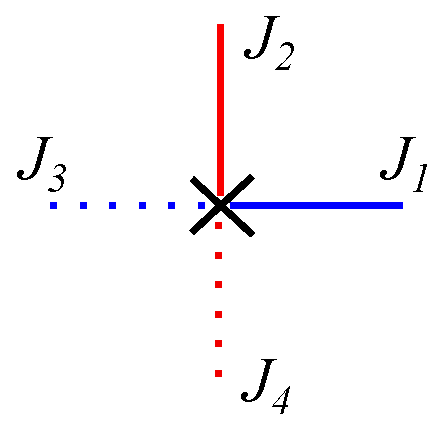
\includegraphics[width=0.7\linewidth]{Pictures/point1.eps} \\ а)}
	\end{minipage}
	\hfill
	\begin{minipage}[h]{0.4\linewidth}
		\center{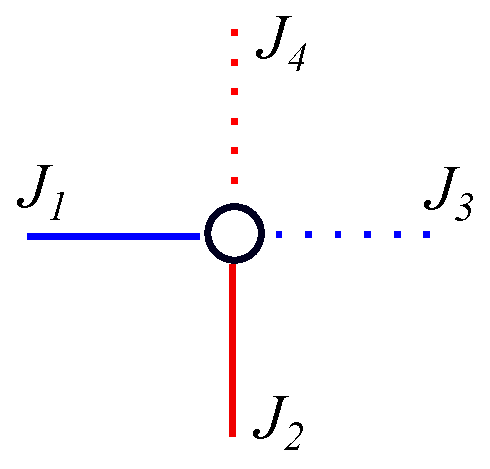
\includegraphics[width=0.7\linewidth]{Pictures/point2.eps} \\ б)}
	\end{minipage}
	\caption{Два вида узлов на обобщенной квадратной решетке }
	\label{point}
\end{figure}

В связи с этим, в отличие от обычной квадратной решетки, имеется 8 различных направлений на обобщенной квадратной решетке (рисунок \ref{dirgen}): 4 направления из узла, обозначенного кружком (вверх, вниз, влево, вправо) и 4 направления из узла, обозначенного крестом (вверх, вниз, влево, вправо).

\begin{figure}[h]
	\center{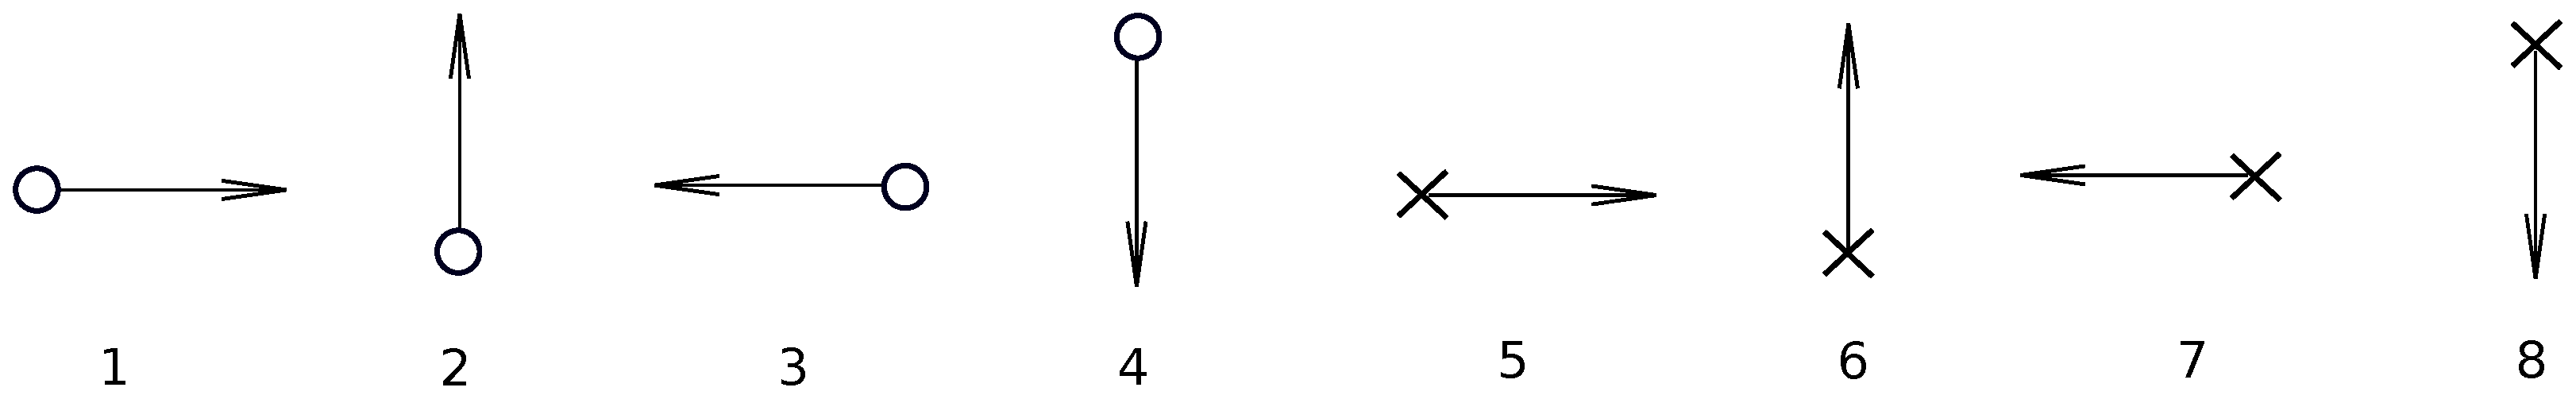
\includegraphics[width=0.9\linewidth]{Pictures/dirgen.eps}}
	\caption{Возможные направления на обобщенной квадратной решетке}
	\label{dirgen}
\end{figure}

Так же как и в случае обычной квадратной решетки, вводится матрица коэффициентов $\Lambda$, а рекурсивные уравнения можно записать в виде
\begin{equation}
W_{r+1}(i, j, \mu) = \sum_{i^{'},\; j^{'},\; \mu^{'}} \Lambda (ij\mu\; |\; i^{'}j^{'}\mu^{'}) W_{r} (i^{'}, j^{'}, \mu^{'}),
\end{equation}

Поскольку существует восемь возможных направлений для движения по решетке, $\Lambda$ представляет собой матрицу $8 \times 8$ с индексами $\mu^{'}$ и $\mu$, графическая интерпретация которой показана на рисунке \ref{matxgen}. 

\begin{figure}[h]
	\center{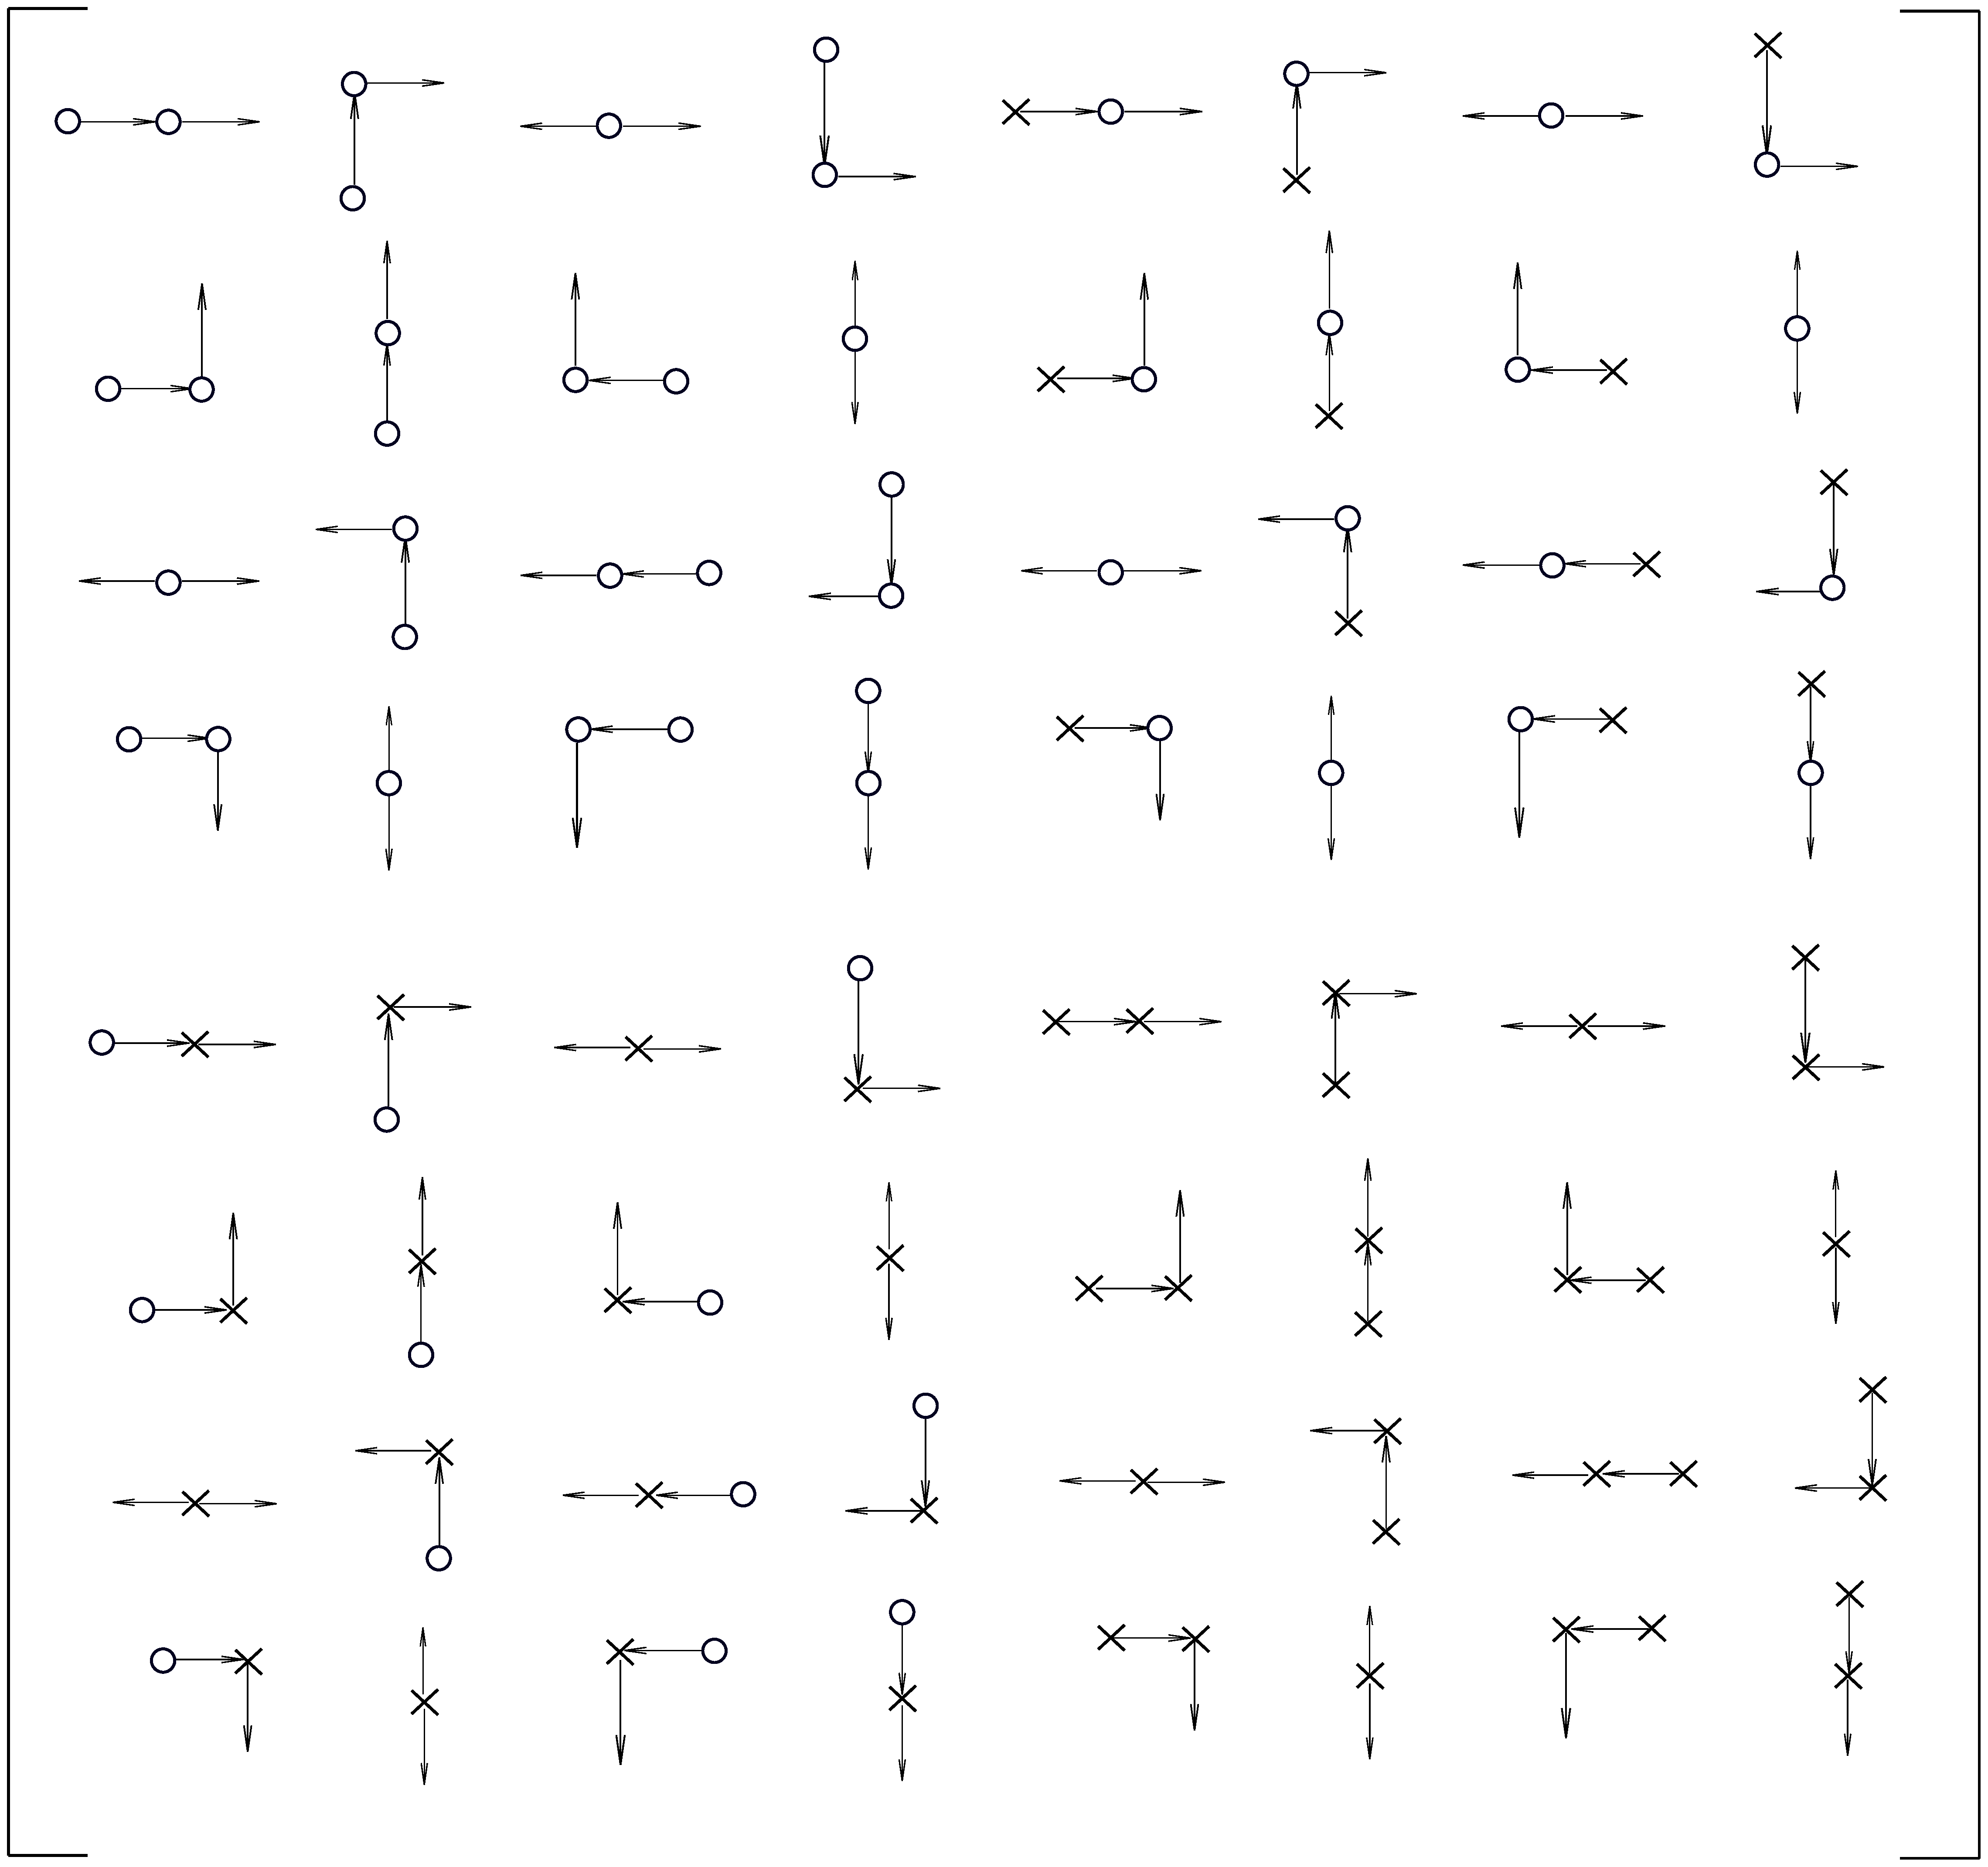
\includegraphics[width=0.7\linewidth]{Pictures/matxgen.eps}}
	\caption{Матричные элементы $\Lambda$}
	\label{matxgen}
\end{figure}

Однако, стоит заметить, что оказывается матрица $\Lambda$ имеет более простой вид, отличный от представленного на рисунке  \ref{matxgen}. Поскольку не существует направлений движения, при которых из узла, обозначенного кружком, происходит переход в такой же узел, а также не существует направлений движения, при которых из узла, обозначенного крестом, происходит переход в похожий узел, все соответствующие матричные элементы равны нулю.

Принимая это во внимание, окончательный вид матрицы коэффициентов $\Lambda$ для обобщенной квадратной решетки записывается в следующем виде
\begin{multline}
\Lambda (p, q, \mu\; |\; p, q, \mu^{'}) = \\ =
\begin{pmatrix}
0 \!\!\!& 0 \!\!\!& 0 \!\!\!& 0\!\!\! & v \epsilon^{-p} \!\!\!& u \alpha^{-1} \epsilon^{-q} \!\!\!& 0 \!\!\!& t \alpha \epsilon^{q} \!\!\! \\
0 \!\!\!& 0 \!\!\!& 0 \!\!\!& 0 \!\!\!& v \alpha \epsilon^{-p}\!\!\! & u \epsilon^{-q}\!\!\! & w \alpha^{-1} \epsilon^{p}\!\!\! & 0\!\!\! \\
0 \!\!\!& 0 \!\!\!& 0 \!\!\!& 0\!\!\! & 0\!\!\! & u \alpha \epsilon^{-q} \!\!\!& w \epsilon^{p} \!\!\!& t \alpha^{-1} \epsilon^{q}\!\!\!  \\
0 \!\!\!& 0 \!\!\!& 0 \!\!\!& 0\!\!\! & v \alpha^{-1} \epsilon^{-p}\!\!\! & 0 \!\!\!& w \alpha \epsilon^{p} \!\!\!& t \epsilon^{q}\!\!\!  \\
w \epsilon^{-p} \!\!\!& t \alpha^{-1} \epsilon^{-q} \!\!\!& 0\!\!\! & u \alpha \epsilon^{q}\!\!\! & 0\!\!\! & 0\!\!\! & 0\!\!\! & 0\!\!\!  \\
w \alpha \epsilon^{-p}\!\!\! & t \epsilon^{-q} \!\!\!& v \alpha^{-1} \epsilon^{p}\!\!\! & 0 \!\!\!& 0\!\!\! & 0\!\!\! & 0\!\!\! & 0\!\!\! \\
0 \!\!\!& t \alpha \epsilon^{-q}\!\!\! & v \epsilon^{p} \!\!\!& u \alpha^{-1} \epsilon^{q}\!\!\! & 0 \!\!\!& 0\!\!\! & 0\!\!\! & 0 \!\!\! \\
w \alpha^{-1} \epsilon^{-p}\!\!\! & 0\!\!\! & v \alpha \epsilon^{p}\!\!\! & u \epsilon^{q} \!\!\!& 0\!\!\! & 0\!\!\! & 0 \!\!\!& 0 \!\!\!
\end{pmatrix},
\end{multline}
где $\epsilon = e^{2\pi i/L}$ и $\alpha = e^{i\pi/4}$.

В соответствии с алгоритмом комбинаторного метода \cite{vdovichenko1965,vaks1965} устанавливается, что
\begin{equation}
	S = 2^N \prod_{i} (1-\lambda_i)^{1/4} = 2^N	\prod_{p, q} \prod_{s=1}^{8} (1-\lambda_s)^{1/4},
	\label{Sformula}
\end{equation}
где $p=2\pi n_1/L$, $q=2\pi n_2/L$, $\lambda_s(p, q)$ -- собственные значения матрицы $\Lambda(p, q)$.

Произведение собственных значений в выражении~(\ref{Sformula}) равно определителю матрицы $1 - \Lambda$. Вычисляя определитель, получается следующее выражение
\begin{align*}
	\Det(1-\Lambda(p, q))& = D(p, q) =\\&= \left(t^2+u^2\right)
	\left(v^2+w^2\right)+\left(t^2 u^2+1\right) \left(v^2 w^2+1\right)+8 t u v w - \\&- 2 \cos (\omega_1-\omega_2) \left( u v \left(t^2-1\right) \left(w^2-1\right)+t w \left(u^2-1\right)
	\left(v^2-1\right) \right) - \\&- 2 \cos (\omega_1+\omega_2) \left( u w \left(t^2-1\right) \left(v^2-1\right) + t v
	\left(u^2-1\right) \left(w^2-1\right)\right)-\\&- 2 v w \left(t^2-1\right) \left(u^2-1\right) \cos \omega_1 - 2 t u \left(v^2-1\right) \left(w^2-1\right) \cos \omega_2,\\ \omega_1 &= \frac{2\pi p}{L}, \omega_2 = \frac{2\pi q}{L}.
\end{align*}

В результате, выражение для свободной энергии (приходящейся на один узел) обобщенной модели Изинга на квадратной решетке с двумя трансляциями в горизонтальном и вертикальном направлениях имеет следующий вид

\begin{multline}
	F(T) = -T \ln Z = -T\ln \lambda_g =  -\ln 2 - \ln \ch \Big(\frac{J_1}{T}\Big) - \ln \ch \Big(\frac{J_2}{T}\Big) - \ln \ch \Big(\frac{J_3}{T}\Big) - \ln \ch \Big(\frac{J_4}{T}\Big) -\\- \frac{T}{4\pi^2} \int_{0}^{2\pi} \int_{0}^{2\pi} \frac{1}{4} \ln D(\omega_1, \omega_2) d\omega_1 d\omega_2.
\end{multline}

Путем несложных преобразований в конечном итоге получается точное аналитическое решение обобщенной модели Изинга на квадратной решетке, совпадающее с решением, приведенным Сиози в статье~\cite{syozi1972}
\begin{multline}
\ln \frac{\lambda_g}{2} = \frac{1}{16 \pi^2} \int_{0}^{2\pi} \int_{0}^{2\pi} \ln \bigg[\frac{1}{2} \bigg( \ch 2K_1 \ch 2K_2 \ch 2K_3 \ch 2K_4 + \\
+ \sh 2K_1 \sh 2K_2 \sh 2K_3 \sh 2K_4 + 1 - \sh 2K_1 \sh 2K_3 \cos (\omega_1 + \omega_2)  - \\ - \sh 2 K_2 \sh 2 K_4 \cos (\omega_1 - \omega_2)  - (\sh 2 K_1 \sh 2 K_4 + \sh 2 K_2 \sh 2 K_3) \cos \omega_1  - \\ - (\sh 2 K_1 \sh 2 K_2 + \sh 2 K_3 \sh 2 K_4) \cos \omega_2 \bigg) \bigg] d\omega_1 d\omega_2,
\end{multline}
где $K_1 = J_1/T$, $K_2 = J_2/T$, $K_3 = J_3/T$, $K_4 = J_4/T$. 

\section{Термодинамические и фрустрационные особенности обобщенной модели Изинга на квадратной решетке}

Обобщенная модель Изинга, в отличие от обычной, привлекательна тем, что позволяет задавать различные обменные взаимодействия между парами спинов, не только по значению, но и по знаку. В данной работе имеется 4 обменных взаимодействия: $J_1$, $J_2$, $J_3$ и $J_4$. Это означает, что существует $2^4 = 16$ различных комбинаций задания знаков между спинами. А вариантов обменных взаимодействий с различными значениями еще больше... Поэтому, для начала рассматриваются обменные взаимодействия с различными знаками при условии, что их модули равны единице: $|J_1| = |J_2| = |J_3| = |J_4| = 1$. В дальнейшем в тексте обменное взаимодействие с положительным знаком ($"+"$) обозначается как ферромагнитное, а с отрицательным знаком ($"−"$) — как антиферромагнитное.

\begin{align*}
 	&1) +\;+\;+\;+\;, \qquad   5) +\;-\;+\;+\;, \qquad	 \;\;9) -\;+\;+\;+\;, \qquad	 13) -\;-\;+\;+\;, \\
	&2) +\;+\;+\;-\;, \qquad  6) +\;-\;+\;-\;, \qquad	 10) -\;+\;+\;-\;, \qquad	 14) -\;-\;+\;-\;, \\
	&3) +\;+\;-\;+\;, \qquad  7) +\;-\;-\;+\;, \qquad  11) -\;+\;-\;+\;, \qquad	 15) -\;-\;-\;+\;, \\
	&4) +\;+\;-\;-\;, \qquad  8) +\;-\;-\;-\;, \qquad	 12) -\;+\;-\;-\;, \qquad	 16) -\;-\;-\;-\;.
\end{align*}

Случаи, отмеченные номерами $1), 16)$ вместе с $|J_1| = |J_2| = |J_3| = |J_4| = 1$ очевидно дают обычную (необобщенную) квадратную решетку~\cite{onsager1941}, с температурными зависимостями энтропии и теплоемкостью, указанных на рисунке~\ref{SimpleSquareLattice}. Те же температурные зависимости дают случаи, отмеченные номерами $4), 6), 7), 10), 11)$ и $13)$. Эти случаи не приводят к фрустрациям, а все потому что спины на квадратной решетке можно расположить таким образом, чтобы удовлетворить всем обменным взаимодействиям.

\begin{figure}[h]
	\begin{minipage}[h]{0.5\linewidth}
		\center{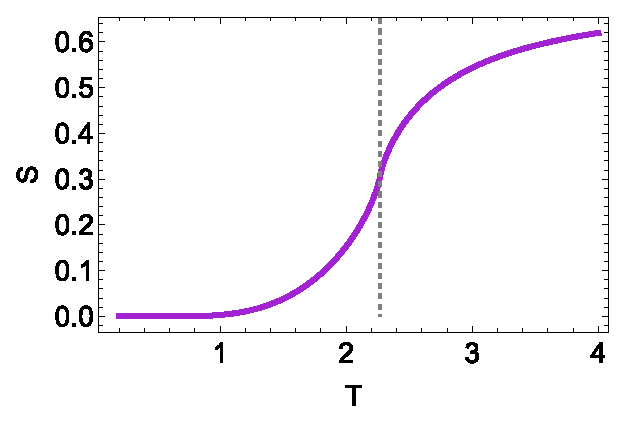
\includegraphics[width=1\linewidth]{Pictures/squareLatticeS.eps} \\ а)}
	\end{minipage}
	\hfill
	\begin{minipage}[h]{0.5\linewidth}
		\center{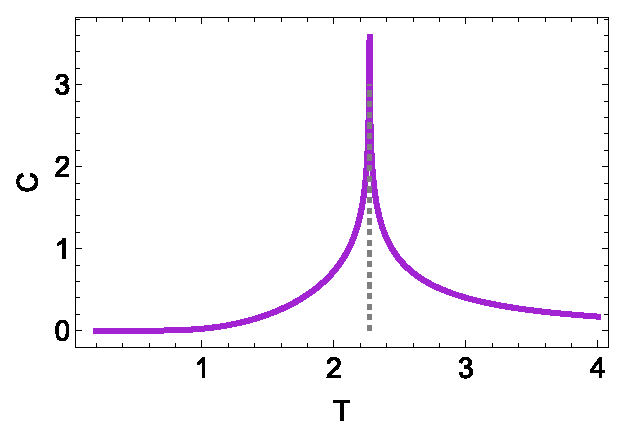
\includegraphics[width=1\linewidth]{Pictures/squareLatticeC.eps} \\ б)}
	\end{minipage}
	\caption{Температурные зависимости обычной квадратной решетки: а) энтропия, б) теплоемкость. Пунктирной линией обозначена температура перехода квадратной решетки: $T_c = 2/(\ln(1+\sqrt{2}))\approx 2.2692$.}
	\label{SimpleSquareLattice}
\end{figure}

Фрустрацию можно получить, если положить одно из взаимодействий антиферромагнитным, а остальные будут ферромагнитными (или, наоборот, одно из взаимодействий ферромагнитно, а другие антиферромагнитны). И неважно какое взаимодействие будет антиферромагнитным (или, наоборот, ферромагнитным). К таким вариантам относятся оставшиеся случаи из списка: $2), 3), 5), 8), 9), 12), 14)$ и $15)$.

\begin{figure}[h]
	\begin{minipage}[h]{0.5\linewidth}
		\center{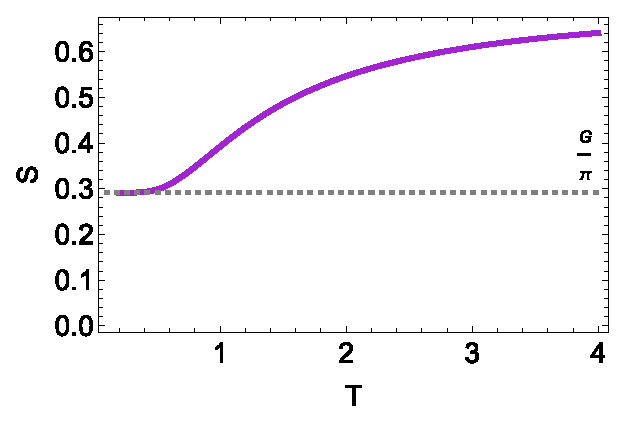
\includegraphics[width=1\linewidth]{Pictures/catalanS.eps} \\ а)}
	\end{minipage}
	\hfill
	\begin{minipage}[h]{0.5\linewidth}
		\center{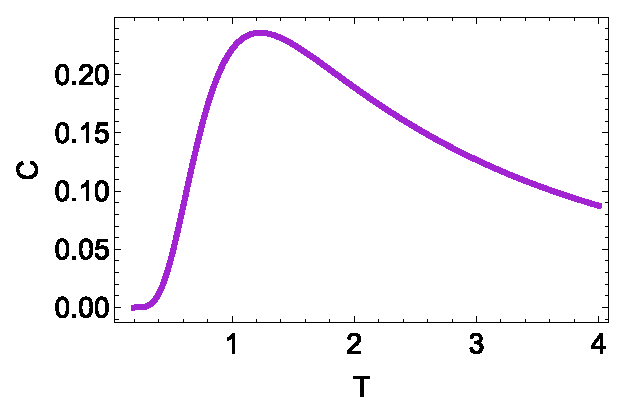
\includegraphics[width=1\linewidth]{Pictures/catalanC.eps} \\ б)}
	\end{minipage}
	\caption{Температурные зависимости обобщенной квадратной решетки c одним ферромагнитным (или антиферромагнитным) взаимодействием и тремя антиферромагнитными (или ферромагнитными) взаимодействиями: а) энтропия, б) теплоемкость. Пунктирной линией обозначена нуль-температурная энтропия: $S_{T\rightarrow 0} = G/\pi\approx 0.29156$, где $G$ --- постоянная Каталана.}
	\label{Catalan}
\end{figure}

При таком выборе знаков обменных взаимодействий спины на квадратной решетке уже не могут удовлетворить всем взаимодействиям, возникает фрустрация, а энтропия при стремлении температуры к нулю оказывается не равной нулю (рис. \ref{Catalan}а), а теплоемкость вместо острого онзагеровского пика принимает куполообразный вид (рис. \ref{Catalan}б). Значение нуль-температурной энтропии найдено по формуле $S = \ln \lambda + T \frac{d}{dT}\ln \lambda$ в виде двукратного определенного интеграла:
\begin{equation*}
	\frac{1}{16\pi^2}\int_{0}^{2\pi}\int_{0}^{2\pi} \ln (4 \sin \beta \cdot \sin \alpha + 4) d\alpha d\beta = 0.29156\dots
\end{equation*}

С помощью несложных алгебраических выкладок оно выражается в виде частного двух математических констант
\begin{equation}
S_{T\rightarrow 0} = \frac{G}{\pi} = 0.29156\dots,
\label{g}
\end{equation} 
где $G$ --- постоянная Каталана, важнейшая константа в теории чисел и в комбинаторике. Любопытно отметить, что в противоположном (полностью ферромагнитном) случае, когда  $J_1 = J_2 = J_3 = J_4 = 1$, величина главного собственного значения трансфер-матрицы Крамерса--Ваннье в точке фазового перехода выражается через те же две константы, что и 
нуль-температурная энтропия в антиферромагнитном случае, а именно: 
\begin{equation}
	\lambda = \sqrt{2} \exp{\Big(\frac{2G}{\pi}\Big)}
\end{equation}
и равна $2.5337373$.

Выполняя зануление одного из четырех обменных взаимодействий, положив $J_4 = 0$, при этом сохраняется условие $|J_1| = |J_2| = |J_3| = 1$. В таком случае образуется восемь вариантов выбора знаков взаимодействий между спинами.

\begin{align*}
	&1) +\;+\;+\;0, \qquad   5) -\;+\;+\;0, \\
	&2) +\;+\;-\;0, \qquad  6) -\;+\;-\;0, \\
	&3) +\;-\;+\;0, \qquad  7) -\;-\;+\;0, \\
	&4) +\;-\;-\;0, \qquad  8) -\;-\;-\;0.
\end{align*}

При занулении одного из взаимодействий на обобщенной квадратной решетке получается гексагональная решетка. Это можно проиллюстрировать, рассмотрев рисунок~\ref{hexTranf}. Действительно, при занулении, например, взаимодействия $J_4$, формируется решетка типа <<кирпичная кладка>>, которая топологически эквивалентна гексагональной решетке. Аналогичное преобразование возможно для любого из четырех взаимодействий на обобщенной квадратной решетке, что приводит к гексагональной решетке. Таким образом, количество вариантов выбора знаков взаимодействий ограничивается восемью.

\begin{figure}[h]
	\center{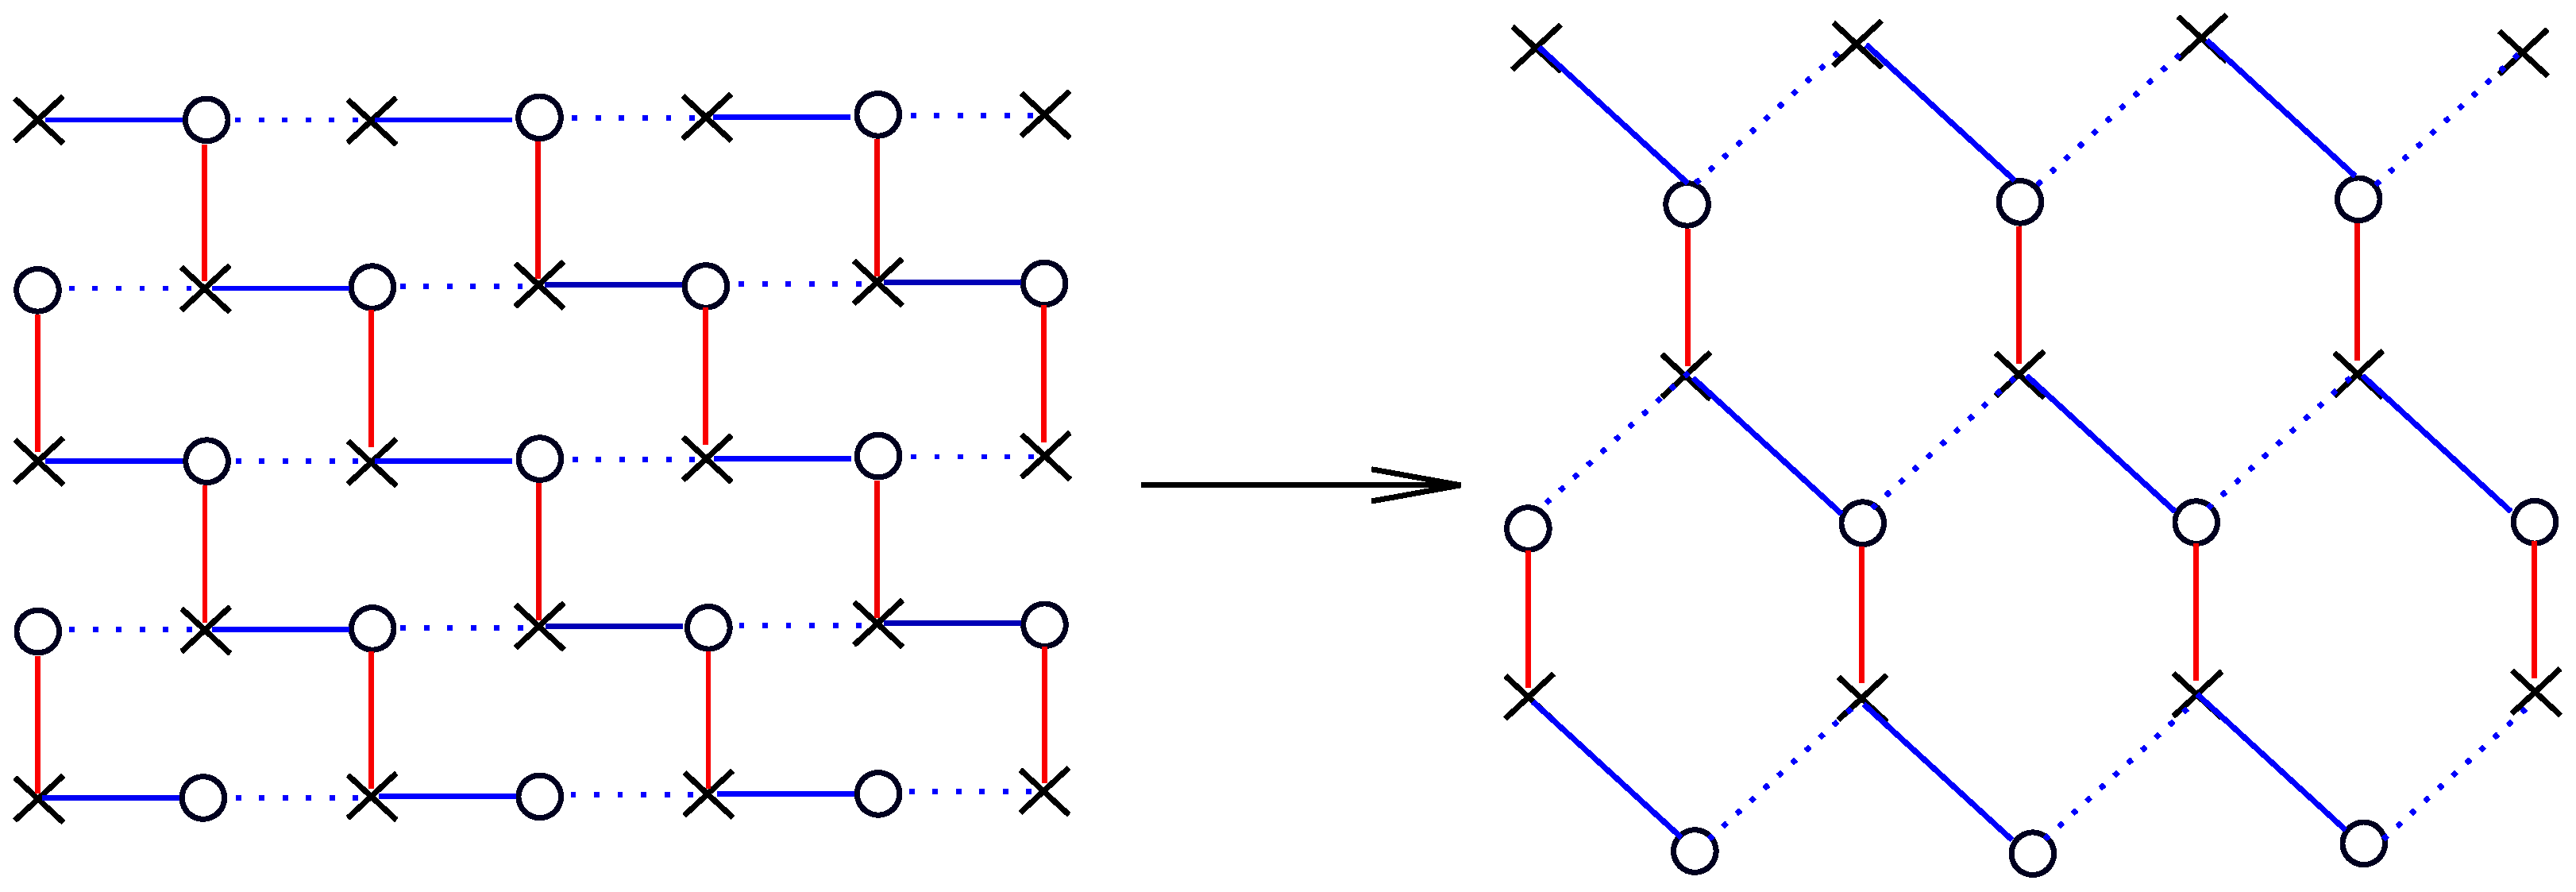
\includegraphics[width=1\linewidth]{Pictures/hex.eps}}
	\caption{При $J_4 = 0$ обобщенная квадратная решетка превращается в так называемую кирпичную кладку, которая топологически эквивалентна гексагональной решетке}
	\label{hexTranf}
\end{figure}

При исследовании различных вариантов выбора знаков взаимодействий, установлено, что все они приводят к одинаковым температурным зависимостям энтропии и теплоемкости, представленным на рисунке~\ref{Hex}. Это объясняется тем, что, как известно~\cite{houtapell1950}, гексагональная решетка при любом выборе знаков взаимодействий не обладает фрустрациями.

\begin{figure}[h]
	\begin{minipage}[h]{0.5\linewidth}
		\center{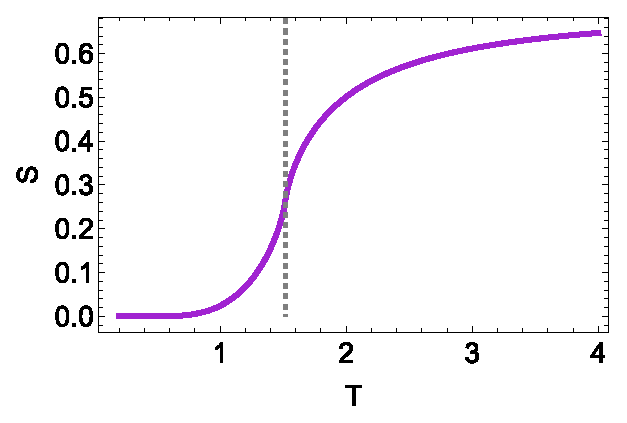
\includegraphics[width=1\linewidth]{Pictures/hexLatticeS.eps} \\ а)}
	\end{minipage}
	\hfill
	\begin{minipage}[h]{0.5\linewidth}
		\center{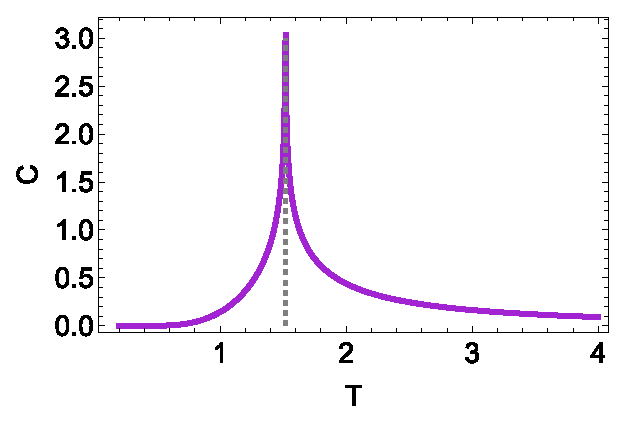
\includegraphics[width=1\linewidth]{Pictures/hexLatticeC.eps} \\ б)}
	\end{minipage}
	\caption{Температурные зависимости обобщенной квадратной решетки с тремя ненулевыми и одним нулевым взаимодействиями (гексагональная решетка): а) энтропия, б) теплоемкость. Пунктирной линией обозначена температура перехода гексагональной решетки: $T_c = 2/(\ln(2+\sqrt{3}))\approx 1.5187$.}
	\label{Hex}
\end{figure}

\begin{figure}[h]
	\begin{minipage}{0.45\linewidth}
		\center{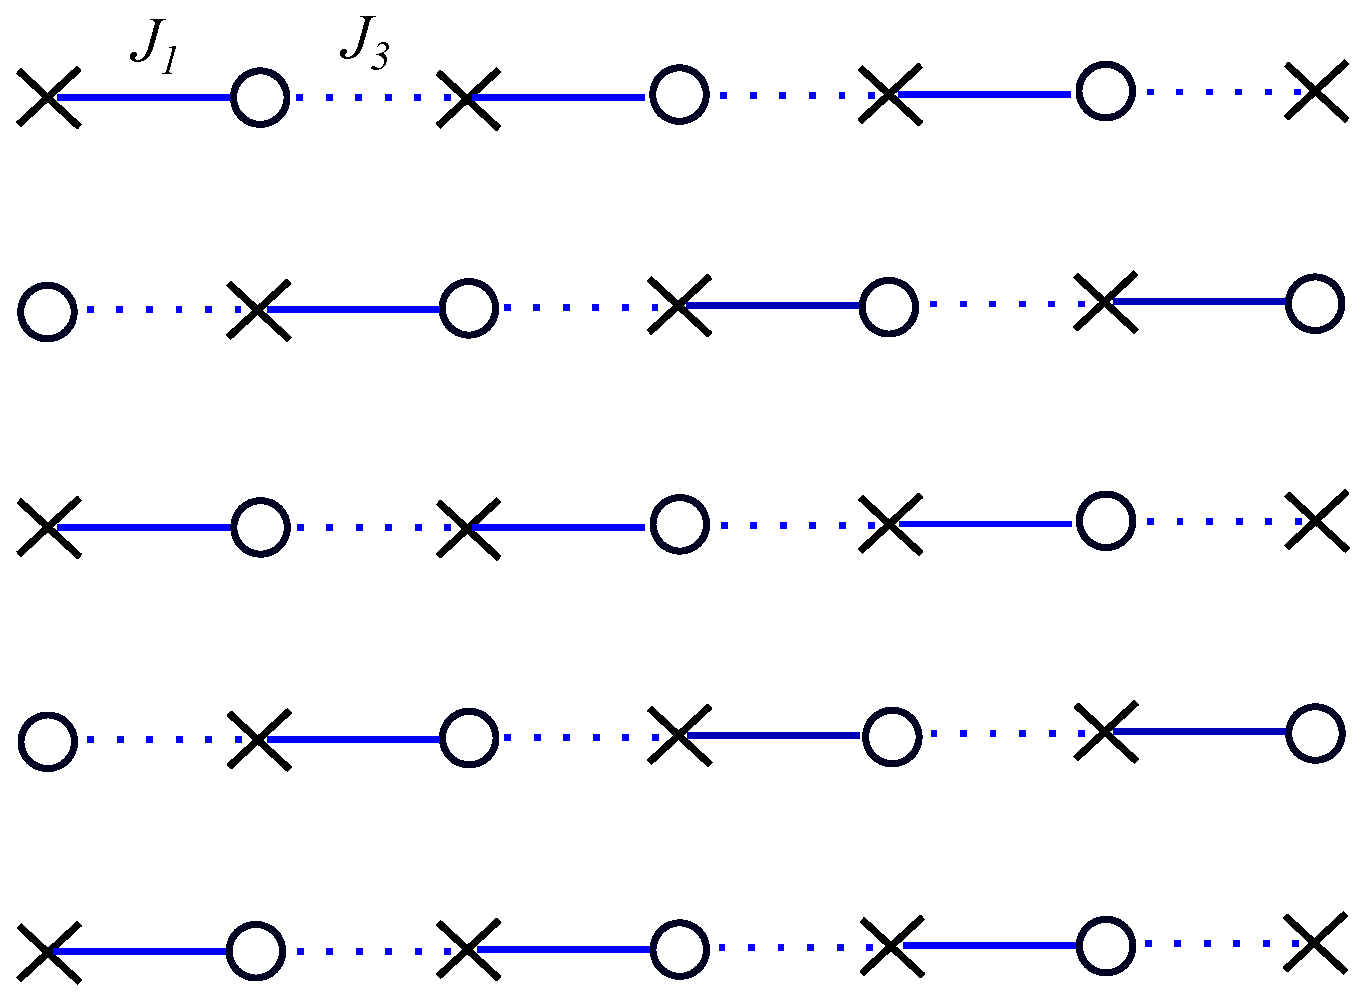
\includegraphics[width=1\linewidth]{Pictures/linear1.eps} \\ а)}
	\end{minipage}
	\hfill
	\begin{minipage}{0.45\linewidth}
		\center{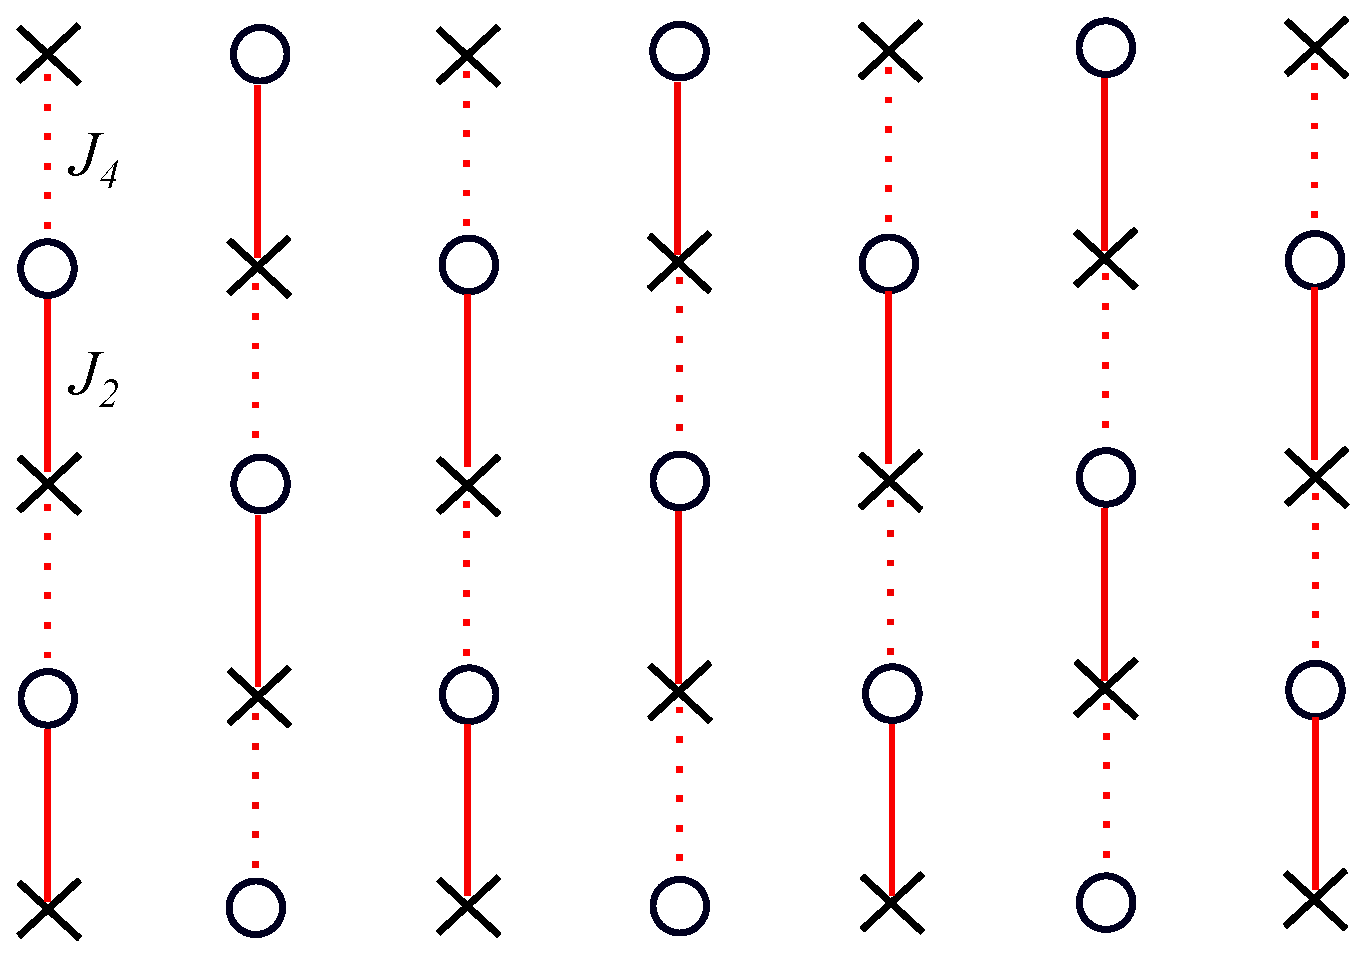
\includegraphics[width=1\linewidth]{Pictures/linear2.eps} \\ б)}
	\end{minipage}
	\vfill
	\begin{minipage}{0.45\linewidth}
		\center{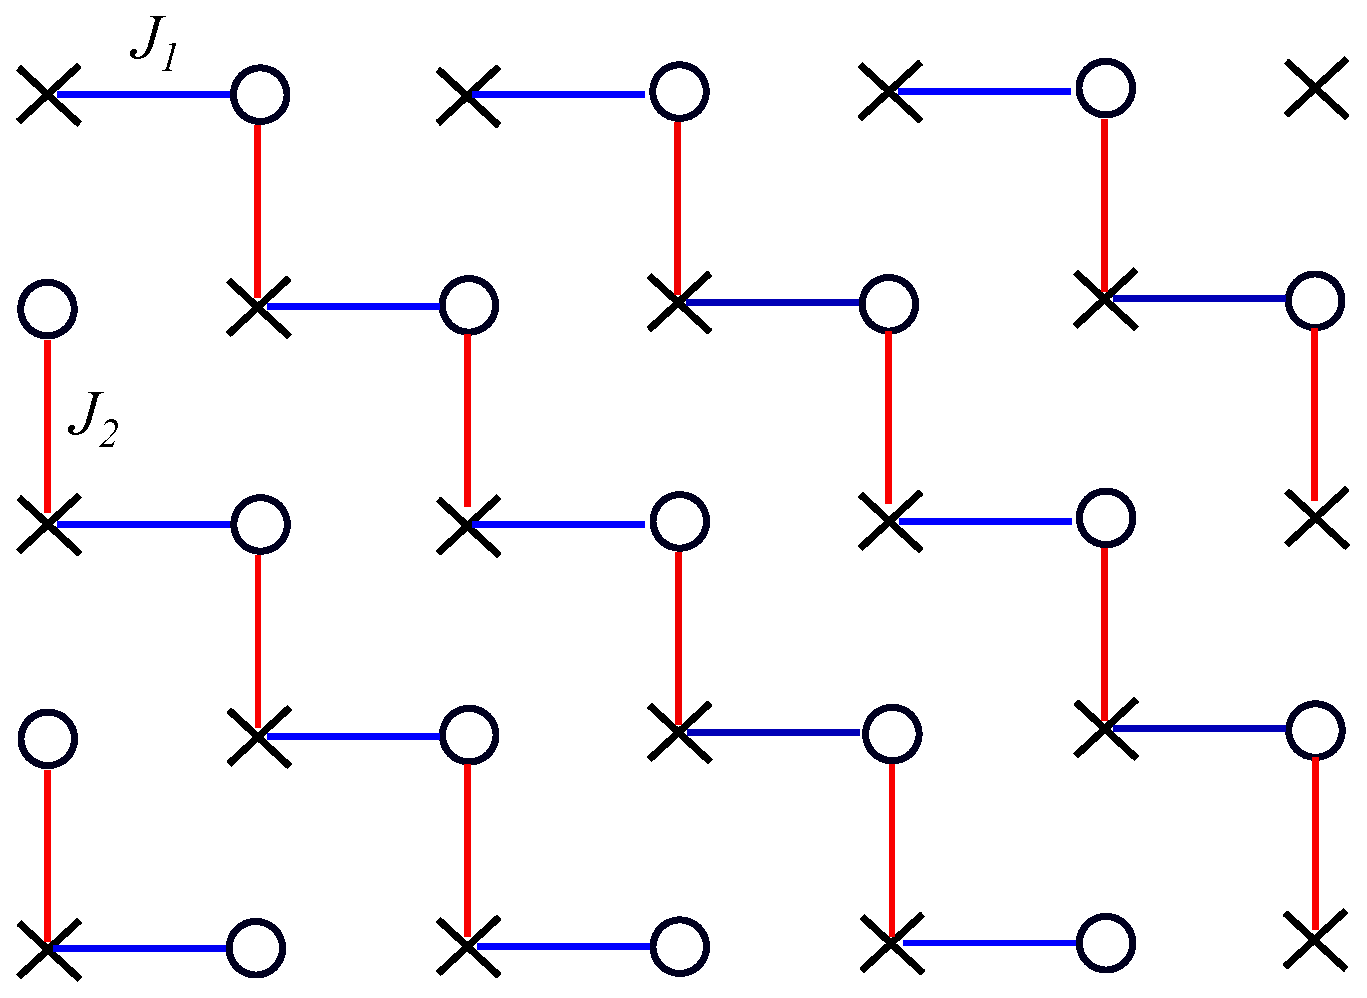
\includegraphics[width=1\linewidth]{Pictures/linear3.eps} \\ в)}
	\end{minipage}
	\hfill
	\begin{minipage}{0.45\linewidth}
		\center{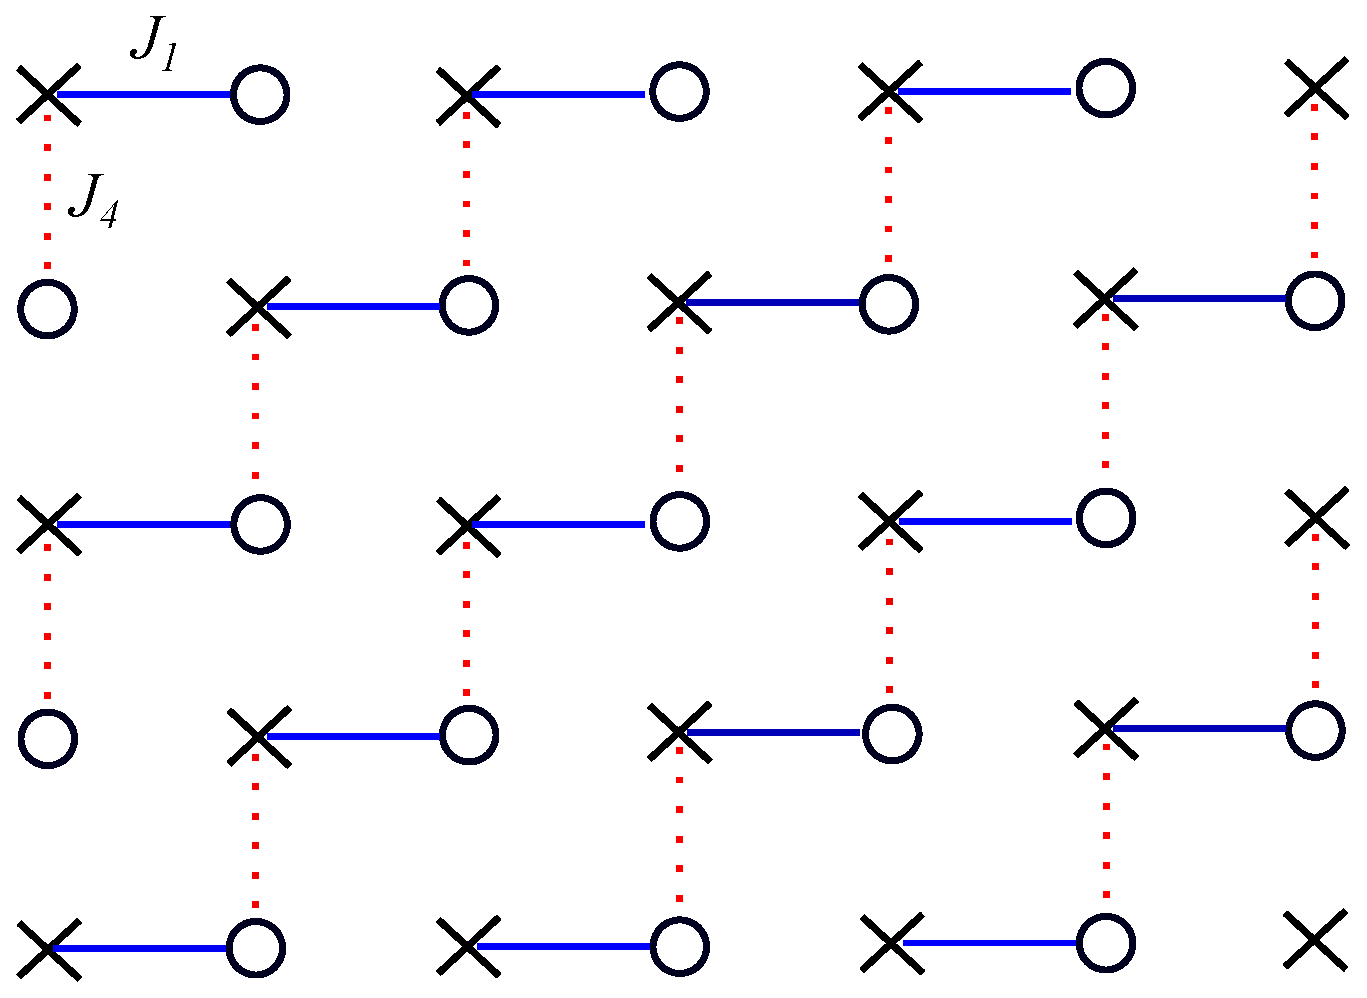
\includegraphics[width=1\linewidth]{Pictures/linear4.eps} \\ г)}	
	\end{minipage}
	\caption{а) и б) <<Прямые>> цепочки, в) и г) Цепочки <<лестничного>> типа.}
	\label{linearChains}
\end{figure}

При занулении сразу двух обменных взаимодействия на обобщенной квадратной решетке получается линейная цепочка, причем существуют различные ее варианты. К ним относятся так называемые <<прямые>> цепочки (рис.~\ref{linearChains}а и рис.~\ref{linearChains}б) и цепочки <<лестничного>> типа (рис.~\ref{linearChains}в и рис.~\ref{linearChains}г). Несмотря на различия в структуре, все эти цепочки демонстрируют одинаковые температурные зависимости энтропии и теплоемкости (рис.~\ref{Linear}). Как известно~\cite{mussardo2010}, любая линейная цепочка не обнаруживает точки перехода, за исключением $T=0$.

\begin{figure}[h]
	\begin{minipage}[h]{0.5\linewidth}
		\center{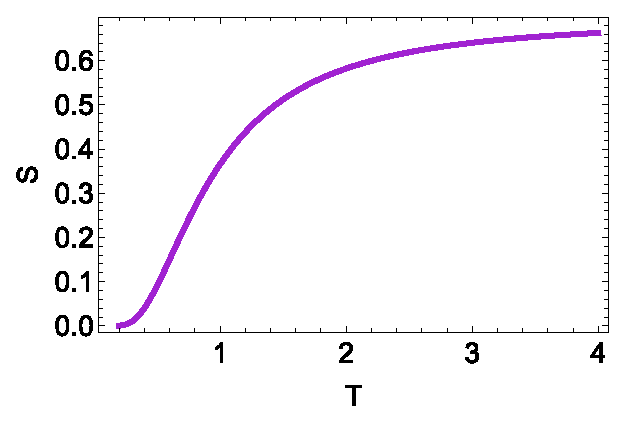
\includegraphics[width=1\linewidth]{Pictures/linearS.eps} \\ а)}
	\end{minipage}
	\hfill
	\begin{minipage}[h]{0.5\linewidth}
		\center{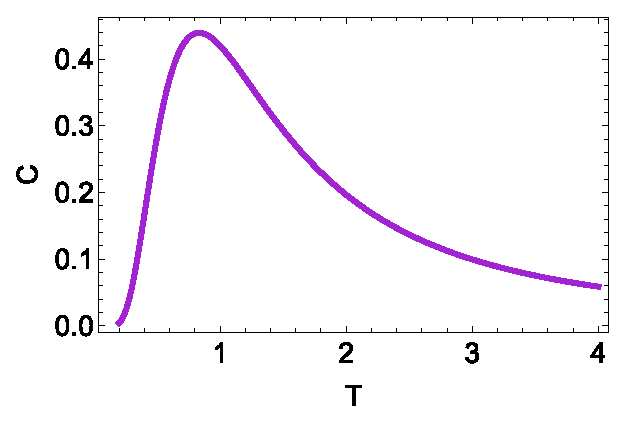
\includegraphics[width=1\linewidth]{Pictures/linearC.eps} \\ б)}
	\end{minipage}
	\caption{Температурные зависимости обобщенной квадратной решетки с двумя ненулевыми и двумя нулевыми взаимодействиями (линейная цепочка): а) энтропия, б) теплоемкость.}
	\label{Linear}
\end{figure}

При занулении трех из четырех обменных взаимодействий, например, $J_2 = J_3 = J_4 = 0$, получается решетка димеров, которая, в отличие от предыдущих случаев, является фрустрированной. В этом случае нуль-температурная энтропия принимает значение $\ln 2/2$, что отражает наличие вырожденного основного состояния и остаточной энтропии.

\begin{figure}[h]
	\center{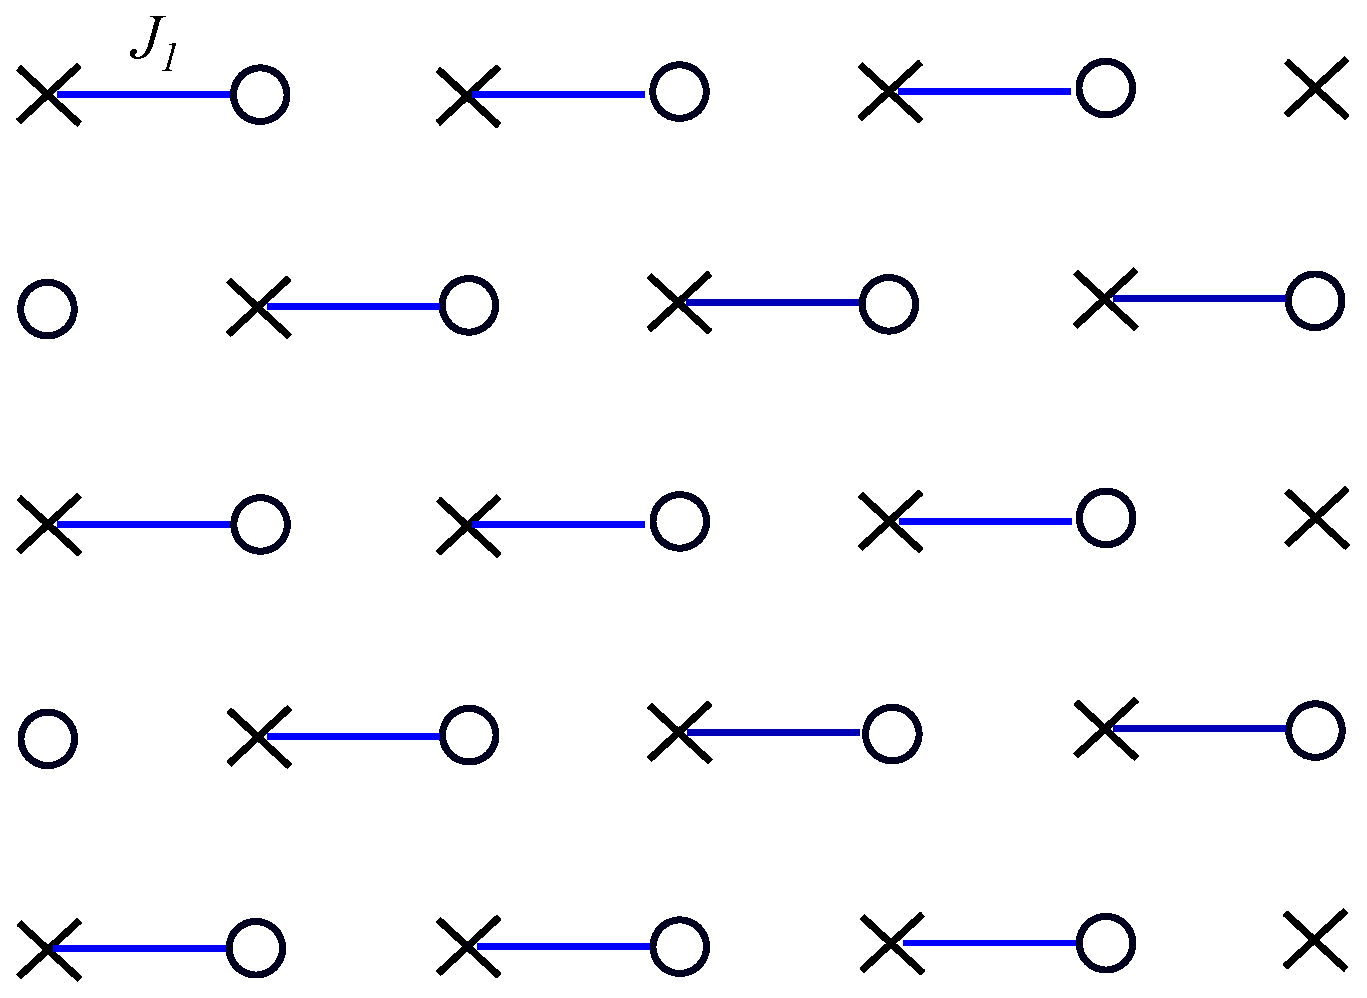
\includegraphics[width=0.45\linewidth]{Pictures/dimers.eps}}
	\caption{Решетка димеров, получаемая из обобщенной квадратной решетки, занулением любых трех взаимодействий, здесь $J_2 = J_3 = J_4 = 0$.}
	\label{dimerLattice}
\end{figure}

Взаимодействие между спинами в одном димере может быть либо ферромагнитным (спины параллельны), либо антиферромагнитным (спины антипараллельны). Количество таких пар, связанных спинов равно $N/2$, что объясняет появление двойки в знаменателе формулы для нуль-температурной энтропии. Поскольку пары спинов не влияют друг на друга, направление спинов в любой паре не коррелирует с направлением спинов соседних пар. Температурные зависимости энтропии и теплоемкости представлены на рисунке~\ref{Dimers}. Аналогичные зависимости возникают при занулении любых трех взаимодействий на обобщенной квадратной решетке, независимо от знака оставшегося взаимодействия (антиферромагнитного или ферромагнитного).

\begin{figure}[h]
	\begin{minipage}[h]{0.5\linewidth}
		\center{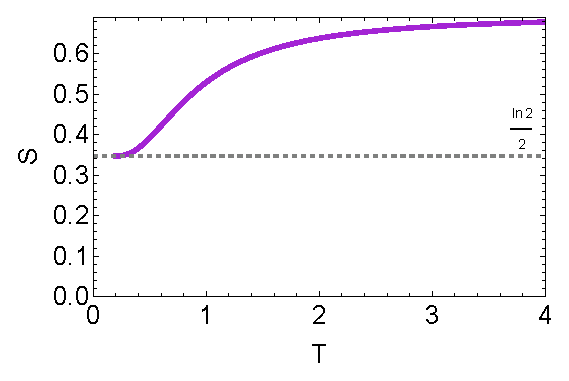
\includegraphics[width=1\linewidth]{Pictures/dimersS.eps} \\ а)}
	\end{minipage}
	\hfill
	\begin{minipage}[h]{0.5\linewidth}
		\center{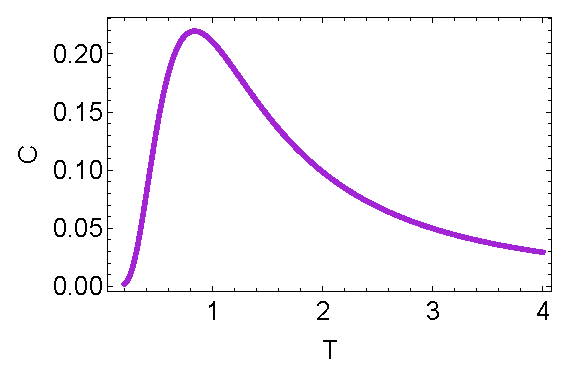
\includegraphics[width=1\linewidth]{Pictures/dimersC.eps} \\ б)}
	\end{minipage}
	\caption{Температурные зависимости обобщенной квадратной решетки с тремя нулевыми и одним ненулевым взаимодействиями (решетка димеров): а) энтропия, б) теплоемкость. Пунктирной линией обозначена нуль-температурная энтропия: $S_{T\rightarrow 0} = \ln 2/2\approx 0.34657$.}
	\label{Dimers}
\end{figure}

В случае, когда все взаимодействия равны нулю $J_1 = J_2 = J_3 = J_4 = 0$, энтропия независимо от температуры принимает постоянное значение $\ln 2$. При рассмотрении энтропии на один узел решетки $S/N$ данный результат отражает, что каждый спин может находиться в одном из двух состояний (спин вверх или спин вниз). Отсутствие взаимодействий между спинами приводит к их свободной ориентации, что соответствует парамагнитному состоянию системы. Такое состояние достигается при стремлении температуры к бесконечности.

Предлагается вернутся к рассмотрению четырех ненулевых обменных взаимодействий на обобщенной квадратной решетке, а именно к случаю $J_1 = -1, J_2 = -1, J_3 = -1, J_4 = 1$ (или $J_1 = 1, J_2 = 1, J_3 = 1, J_4 = -1$). Уже известно, что при таком выборе параметров обменного взаимодействия решетка будет фрустрированной с нуль-температурной энтропией равной $G/\pi$ (рис.~\ref{Catalan}). 

При увеличении ферромагнитного значения $J_4$ при сохранении остальных взаимодействий неизменными, получаемые температурные зависимости энтропии для ряда значений обменных взаимодействий проиллюстрированы на рисунке~\ref{Peak}. На этих графиках наблюдается, что при $J_4>1$ все кривые энтропии сходятся к одному и тому же значению при стремлении температуры к нулю ($T \rightarrow 0$). 

\begin{figure}[h]
	\begin{minipage}[h]{0.5\linewidth}
		\center{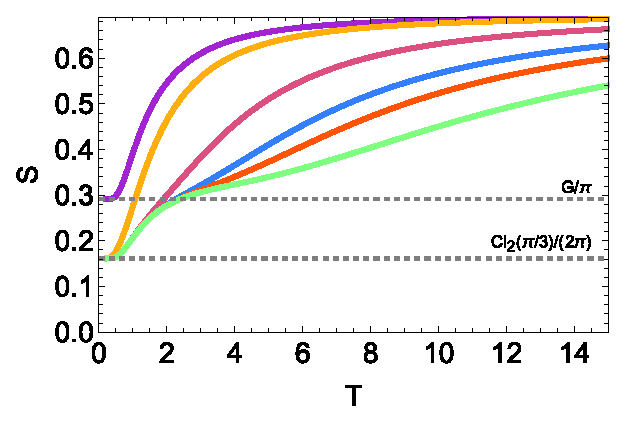
\includegraphics[width=1\linewidth]{Pictures/peakS.eps} \\ а)}
	\end{minipage}
	\hfill
	\begin{minipage}[h]{0.5\linewidth}
		\center{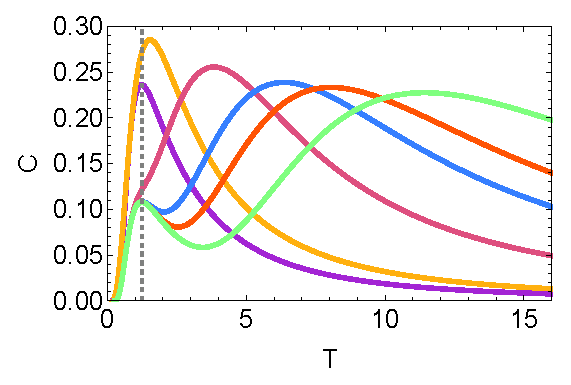
\includegraphics[width=1\linewidth]{Pictures/peakC.eps} \\ б)}
	\end{minipage}
	\caption{Температурные зависимости обобщенной квадратной решетки для различных параметров обменных взаимодействий: фиолетовая кривая --- $J_1 = -1$, $J_2 = -1$, $J_3 = -1$, $J_4 = 1$, желтая кривая --- $J_1 = -1$, $J_2 = -1$, $J_3 = -1$, $J_4 = 2$, розовая кривая --- $J_1 = -1$, $J_2 = -1$, $J_3 = -1$, $J_4 = 5$, синяя кривая --- $J_1 = -1$, $J_2 = -1$, $J_3 = -1$, $J_4 = 8$, красная кривая --- $J_1 = -1$, $J_2 = -1$, $J_3 = -1$, $J_4 = 10$, зеленая кривая --- $J_1 = -1$, $J_2 = -1$, $J_3 = -1$, $J_4 = 14$: а) энтропия. Пунктирными линиями обозначены значения нуль-температурных энтропий: $S_{T\rightarrow 0} = G/\pi\approx 0.29156$, где $G$ --- постоянная Каталана, $S_{T\rightarrow 0} = \frac{1}{2\pi} \Cl_2 (\frac{\pi}{3})\approx0.16153$, где $\Cl_2 (\varphi)$ --- функция Клаузена. б) теплоемкость. Пунктирной линией обозначено положение дополнительного гладкого пика ($T_{peak}\approx1.232$). }
	\label{Peak}
\end{figure}

Установлено, что нуль-температурное значение для энтропий, когда $J_4>1$, выражается в виде    
\begin{equation}
S_{T\rightarrow 0} = \frac{1}{2\pi} \Cl_2 \bigg(\frac{\pi}{3}\bigg)   = 0.16153\dots, 
\label{cl}
\end{equation} 
где  $\Cl_2 (\varphi)$ --- функция Клаузена. Функция Клаузена --- трансцендентная специальная функция одной переменной, которая связана с мнимой частью дилогарифма $\Li_2$
\begin{equation*}
\Cl_2 (\varphi) = \im (\Li_2 (e^{i \varphi})).
\end{equation*}

Кроме того, функция Клаузена может быть записана через различные интегральные представления, которые можно найти в математическом справочниках и статьях (например, \cite{abramowitz_stegun1972, wood1968}).

Интересно то, что постоянную Каталана так же можно выразить через функцию Клаузена~\cite{wood1968}
\begin{equation*}
G = \Cl_2 \bigg(\frac{\pi}{2}\bigg) = \im (\Li_2 (i)),
\end{equation*}

\noindent поэтому фрустрационное значение энтропии в выражении \eqref{g} может быть переписано в виде
\begin{equation}
\frac{G}{\pi} = \frac{1}{\pi} \Cl_2 \bigg(\frac{\pi}{2}\bigg) = 0.29156\dots
\end{equation}

Кроме того, при увеличение ферромагнитного значения $J_4$ наблюдается необычная особенность в поведении теплоемкости, представленная на рисунке~\ref{Peak}. Начиная с $J_4 = 5$ (розовая кривая на рисунке~\ref{Peak}б), формируется дополнительный гладкий пик теплоемкости, тогда как основной широкий пик одновременно растягивается и смещается вправо по температурной оси. При этом положение дополнительного пика остается практически неизменным при дальнейшем увеличении $J_4$, в то время как основной пик теплоемкости продолжает смещаться. Что касается энтропий, то их нуль-температурные значения при $J_4>1$ равны одному и тому же значению $\frac{1}{2\pi} \Cl_2 (\frac{\pi}{3})$. Аналогичные рассуждения применимы и для случая $J_1 = 1, J_2 = 1, J_3 = 1$ при антиферромагнитном увеличении $J_4$.

Наблюдаемое поведение теплоемкости и энтропии при увеличении ферромагнитного взаимодействия $J_4$ в фрустрированной системе представляет собой нетипичный феномен. Появление дополнительного стабильного пика теплоемкости вместе с изменением положения основного пика указывает на сложную перестройку низкотемпературного состояния и возможное возникновение новых корреляционных или квазипериодических структур в системе. Это требует более глубокого теоретического и численного анализа, чтобы понять природу и механизм данной перестройки. Такие исследования могут пролить свет на новые физические эффекты в фрустрированных магнитных системах и расширить представления о термодинамическом поведении моделей с многокомпонентными обменными взаимодействиями.

\begin{figure}[h]
	\begin{minipage}[h]{0.5\linewidth}
		\center{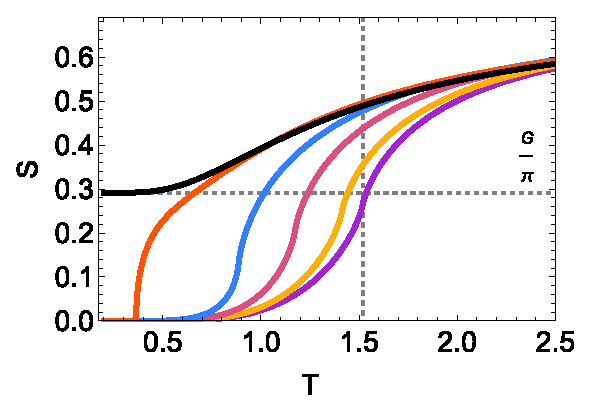
\includegraphics[width=1\linewidth]{Pictures/peak2S.eps} \\ а)}
	\end{minipage}
	\hfill
	\begin{minipage}[h]{0.5\linewidth}
		\center{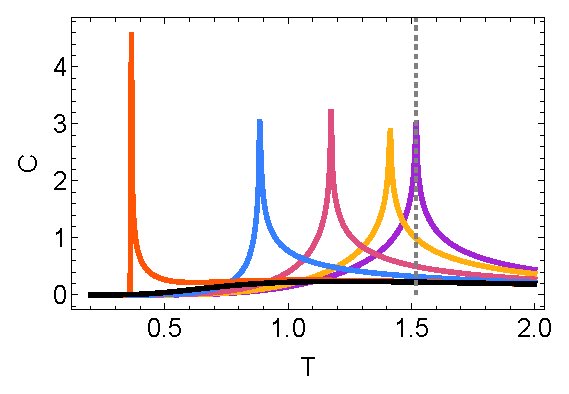
\includegraphics[width=1\linewidth]{Pictures/peak2C.eps} \\ б)}
	\end{minipage}
	\caption{Температурные зависимости обобщенной квадратной решетки для различных параметров обменных взаимодействий: фиолетовая кривая --- $J_1 = -1$, $J_2 = -1$, $J_3 = -1$, $J_4 = 0$, желтая кривая --- $J_1 = -1$, $J_2 = -1$, $J_3 = -1$, $J_4 = 0.1$, розовая кривая --- $J_1 = -1$, $J_2 = -1$, $J_3 = -1$, $J_4 = 0.3$, синяя кривая --- $J_1 = -1$, $J_2 = -1$, $J_3 = -1$, $J_4 = 0.5$, красная кривая --- $J_1 = -1$, $J_2 = -1$, $J_3 = -1$, $J_4 = 0.8$, черная кривая --- $J_1 = -1$, $J_2 = -1$, $J_3 = -1$, $J_4 = 1$: а) энтропия. Пунктирными линиями обозначены значение нуль-температурной энтропии: $S_{T\rightarrow 0} = G/\pi\approx 0.29156$, где $G$ --- постоянная Каталана и значение точки перехода для гексагональной решетки $T_c = 2/(\ln(2+\sqrt{3}))\approx 1.5187$. б) теплоемкость. Пунктирной линией обозначено значение точки перехода для гексагональной решетки $T_c = 2/(\ln(2+\sqrt{3}))\approx 1.5187$. }
	\label{Peak2}
\end{figure}

Рассмотрим поведение системы при приближении к точке фрустрации с обменными взаимодействиями $J_1 = -1$, $J_2 = -1$, $J_3 = -1$, $J_4 = 1$ (черная кривая на рисунке~\ref{Peak2}). Исходно принимаются параметры $J_1 = -1$, $J_2 = -1$, $J_3 = -1$, $J_4 = 0$, что соответствует случаю гексагональной решетки~(см. рис.~\ref{Hex}). Энтропия и теплоемкость для этой решетки представлены фиолетовой кривой на рисунках \ref{Peak2}а и \ref{Peak2}б соответственно. При постепенном увеличении ферромагнитного параметра $J_4$ от $0$ до $1$ на основе рисунков \ref{Peak2}а и \ref{Peak2}б делаются следующие выводы. Во-первых, зависимости теплоемкости имеют форму $\lambda$ -- образных пиков, что свидетельствует о наличии фазовых переходов в точках скачков теплоемкости. Это означает, отсутствие бесконечного числа вырожденных конфигураций с одинаковой энергией, то есть фрустрация отсутствует. Во-вторых, при приближении к точке фрустрации $J_1 = -1$, $J_2 = -1$, $J_3 = -1$, $J_4 = 1$ (черная кривая на рисунке~\ref{Peak2}) наблюдается смещение пиков теплоемкости влево по температурной оси с характерным <<укручением>> левой части теплоемкости.

\begin{figure}[h]
	\begin{minipage}[h]{0.5\linewidth}
		\center{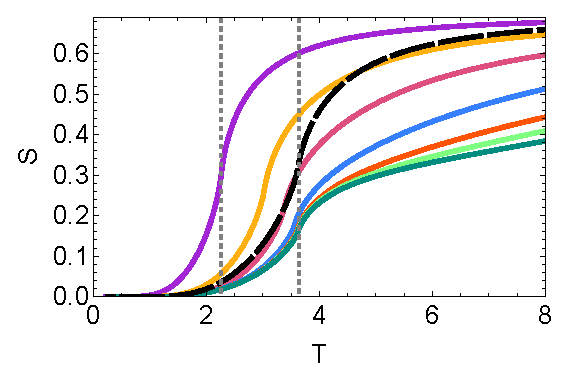
\includegraphics[width=1\linewidth]{Pictures/triangularS.eps} \\ а)}
	\end{minipage}
	\hfill
	\begin{minipage}[h]{0.5\linewidth}
		\center{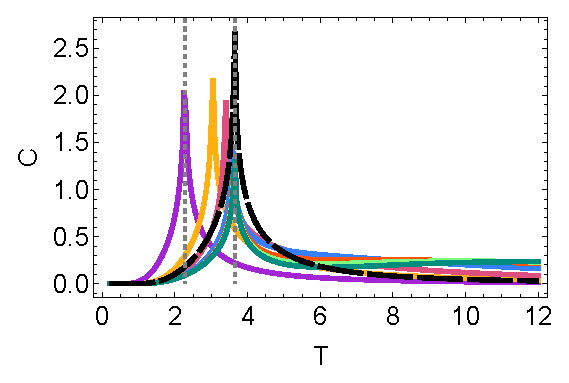
\includegraphics[width=1\linewidth]{Pictures/triangularC.eps} \\ б)}
	\end{minipage}
	\caption{Температурные зависимости обобщенной квадратной решетки для различных параметров обменных взаимодействий: фиолетовая кривая --- $J_1 = 1$, $J_2 = 1$, $J_3 = 1$, $J_4 = 1$, желтая кривая --- $J_1 = 1$, $J_2 = 1$, $J_3 = 1$, $J_4 = 3$, розовая кривая --- $J_1 = 1$, $J_2 = 1$, $J_3 = 1$, $J_4 = 5$, синяя кривая --- $J_1 = 1$, $J_2 = 1$, $J_3 = 1$, $J_4 = 8$, красная кривая --- $J_1 = 1$, $J_2 = 1$, $J_3 = 1$, $J_4 = 11$, зеленая кривая --- $J_1 = 1$, $J_2 = 1$, $J_3 = 1$, $J_4 = 13$, темно-зеленая кривая --- $J_1 = 1$, $J_2 = 1$, $J_3 = 1$, $J_4 = 15$: а) энтропия, б) теплоемкость. Пунктирными линиями обозначены значения точек перехода для квадратной и треугольной решеток соответственно: $T_c = 2/(\ln(1+\sqrt{2}))\approx 2.2692$,  $T_c = 4/\ln 3\approx 3.64096$. Черной пунктирной линией обозначены температурные зависимости энтропии и теплоемкости треугольной решетки с параметрами $J_1 = J_2 = J_3 = 1$.}
	\label{Triangular}
\end{figure}

\begin{figure}[h]
	\center{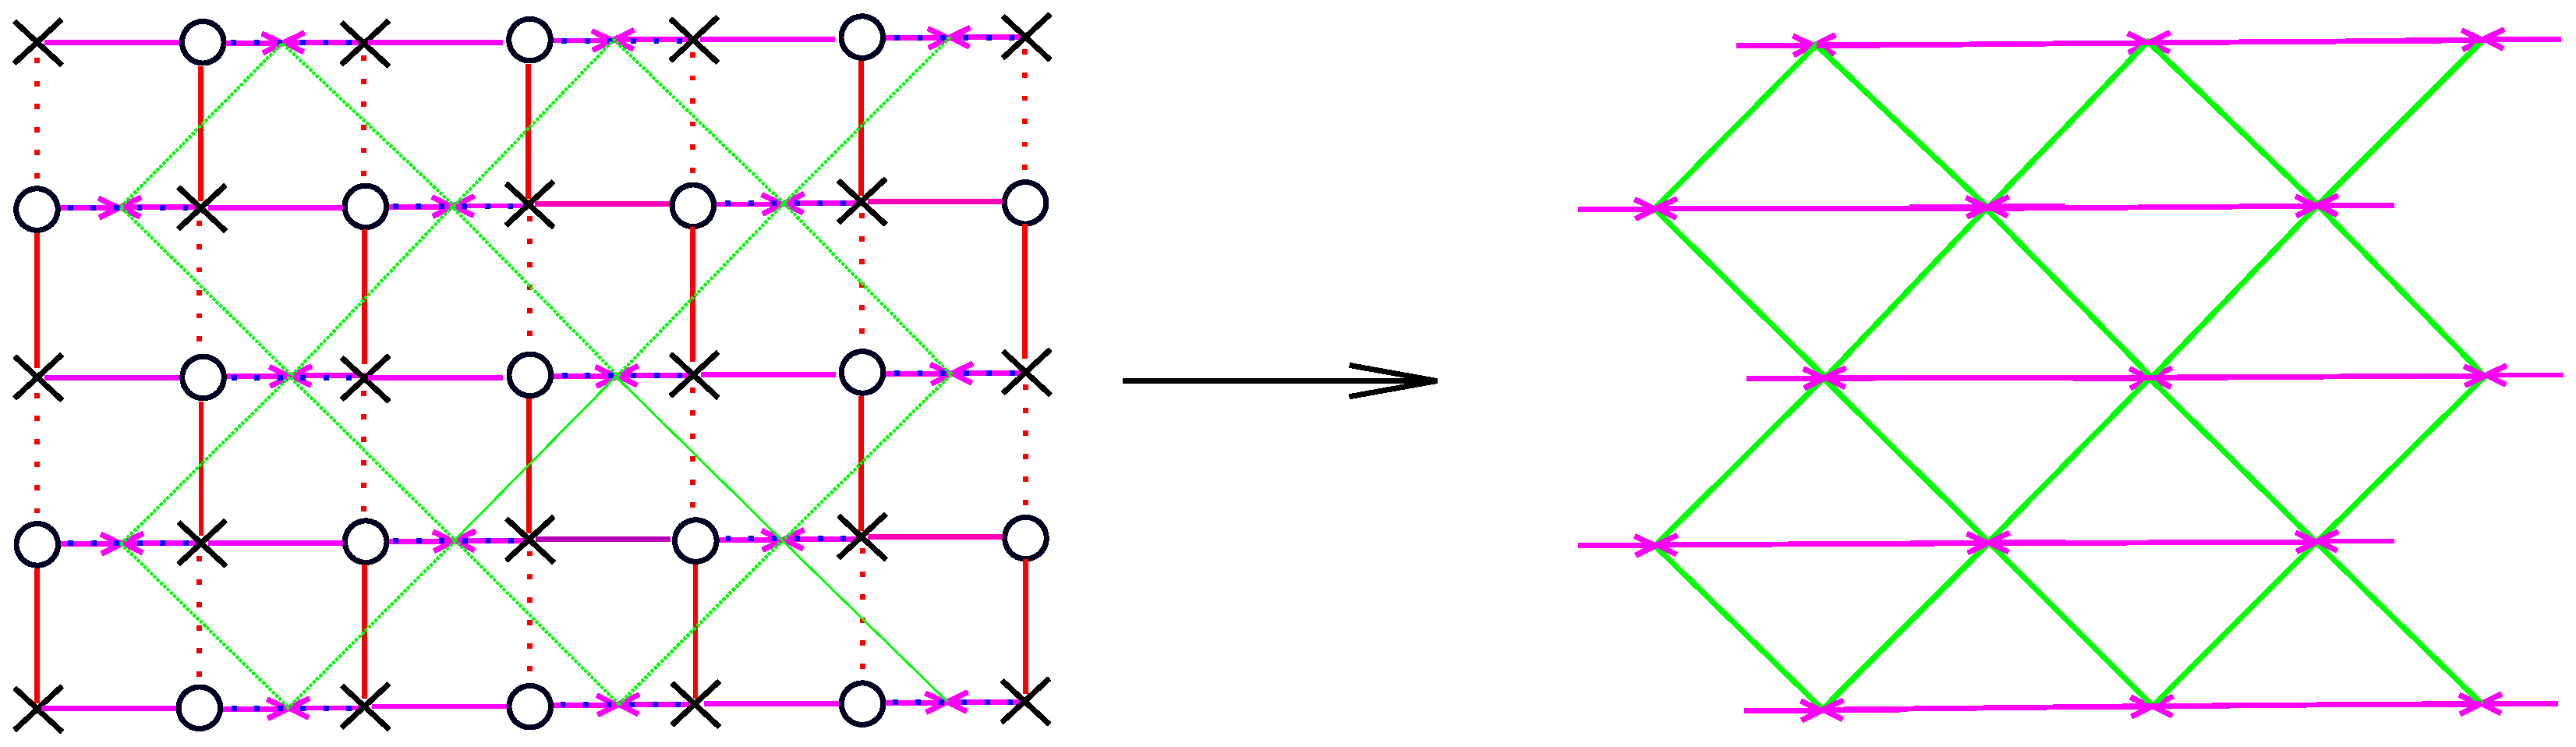
\includegraphics[width=1\linewidth]{Pictures/triag.eps}}
	\caption{Преобразование обобщенной квадратной решетки к треугольной решетке, устремляя одно из обменных взаимодействий к бесконечности}
	\label{triag}
\end{figure}

Далее продемонстрирован еще один частный случай обобщенной квадратной решетки с двумя трансляциями. Пусть параметры обменных взаимодействий равны $J_1 = J_2 = J_3 = J_4 = 1$ (фиолетовая кривая на рисунке~\ref{Triangular}). Этот случай соответствует классической онзагеровской квадратной решетке с температурой фазового перехода $T_c = 2/(\ln (1+\sqrt{2}))$~\cite{kramers_wannier1, kramers_wannier2}. При увеличении ферромагнитного параметра $J_4$, значения энтропии и теплоемкости сходятся к определенной точке перехода, что иллюстрируют рисунки \ref{Triangular}а и \ref{Triangular}б. Эта точка соответствует температуре фазового перехода треугольной решетки $T_c = 4/\ln 3$~\cite{wannier1950}. Треугольная решетка в данном случае может быть получена в пределе, когда одно из взаимодействий стремится к бесконечности. Таким образом, обобщенная квадратная решетка сводится к треугольной решетке. Подтверждением данного факта служит рисунок~\ref{triag}. 

При рассмотрении обобщенной квадратной решетки с параметрами $J_1 = -1, J_2 = -1, J_3 = -1$ и $J_4 > 0$ наблюдалось аналогичное поведение: увеличение значения параметра $J_4$ приводило к трансформации обобщенной квадратной решетки в другую структуру. Однако на практике параметр $J_4$ можно увеличить лишь до некоторого конечного значения, а не до бесконечности. В результате система не переходит в треугольную решетку, а формируется топологически искаженная решетка Кагоме~(см. рис.~\ref{kagomelike}). Такая решетка характеризуется наличием шестиугольников и треугольников различных размеров, в отличие от классической решетки Кагоме, где все треугольники имеют одинаковый размер. 

\begin{figure}[h]
	\center{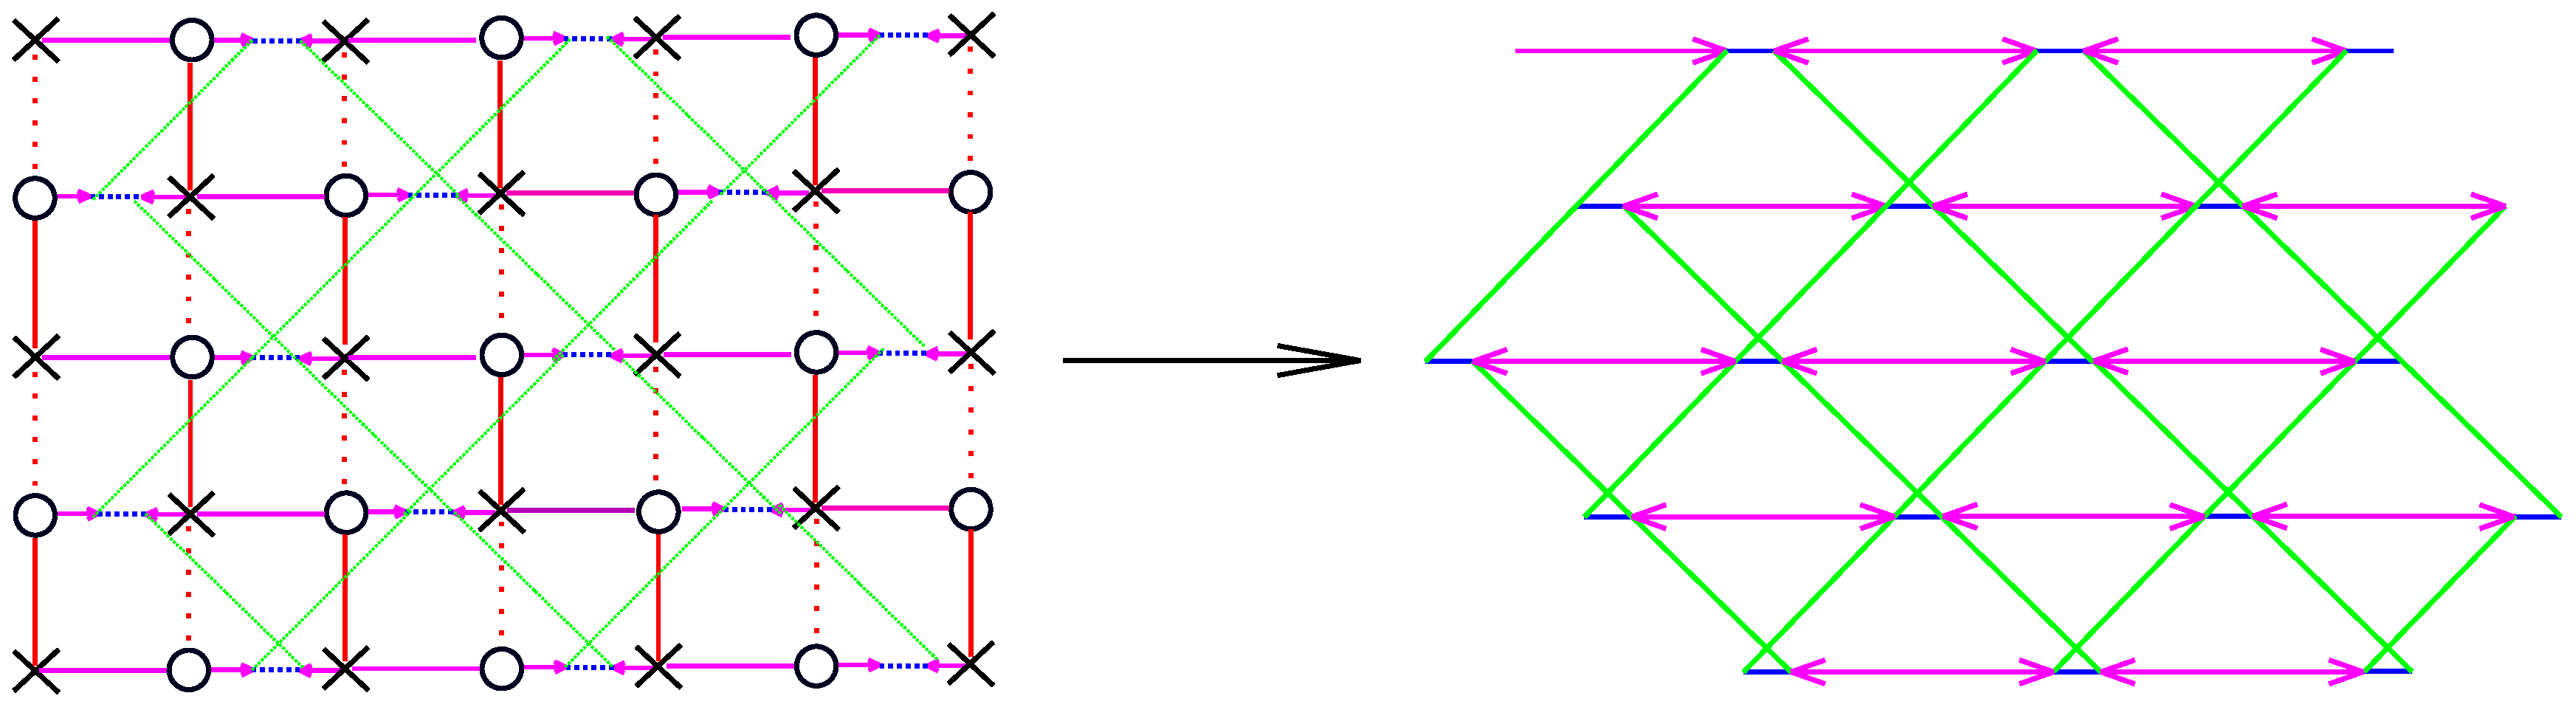
\includegraphics[width=1\linewidth]{Pictures/kagomelike.eps}}
	\caption{Получение искаженной кагоме решетки из обобщенной модели Изинга при конечном увеличении одного из параметров обменного взаимодействия}
	\label{kagomelike}
\end{figure}

Следует отметить, что на данной решетке наблюдается фрустрация при параметрах $J_1 = -1, J_2 =-1, J_3 = -1, J_4 = 1$. При дальнейшем увеличении $J_4$ состояние фрустрации сохраняется, при этом все значения нуль-температурной энтропии совпадают и равны $\frac{1}{2\pi} \Cl_2 (\frac{\pi}{3})$, а теплоемкость демонстрирует дополнительный гладкий пик (см. рис.~\ref{Peak}б).

\section{Замощение шахматной решетки плитками домино}

Помимо классических подходов к решению двумерной модели Изинга, таких как точное аналитическое решение Онзагера и комбинаторные методы, существует альтернативный и весьма мощный метод, известный как метод димеров. Этот метод был существенно развит в работах Кастелайна~\cite{kasteleyn1961, kasteleyn1963_1, kasteleyn1963_2}, Темперли~\cite{temperley1961} и Фишера~\cite{fisher1966}.

Димер — это ребро графа, которое покрывает ровно две соседние вершины. Задача подсчета числа димерных покрытий графа, то есть разбиений множества вершин графа на пары, связанных ребрами, является классической в комбинаторике и статистической механике. Она тесно связана с изучением различных моделей взаимодействующих систем.

Идея применения димерных покрытий к решению модели Изинга возникла из наблюдения, что конфигурации спинов в модели Изинга можно однозначно сопоставить с определенными димерными покрытиями специально построенного графа. Для двумерной модели Изинга на квадратной решетке существует соответствие между конфигурациями спинов и димерными покрытиями некоторого связанного графа, что позволяет свести задачу вычисления статистической суммы модели Изинга к задаче подсчета числа димерных покрытий.

В начале 1960-х годов Кастелайн разработал метод вычисления числа димерных покрытий плоских графов, введя понятие так называемой ориентации Кастелайна. Эта ориентация представляет собой направление ребер графа, обладающее особым свойством: для каждого цикла нечетной длины число ребер, ориентированных в определенном направлении, должно быть нечетным. Благодаря такой ориентации задача подсчета числа димерных покрытий сводится к вычислению определителя специально построенной матрицы смежности графа, что значительно упрощает вычисления.

Независимо от Кастелайна, Фишер совместно с Темперли разработали методы, позволяющие выразить статистическую сумму модели Изинга через задачи подсчета димерных покрытий. Фишер предложил конструкцию, которая переводит исходную задачу Изинга в задачу димеров на так называемом расширенном графе (Fisher graph). В этом графе вершины и ребра модифицированы таким образом, чтобы сохранить всю информацию об исходной модели, что дает возможность применить методы подсчета димерных покрытий к вычислению статистической суммы.

Таким образом, метод димеров является еще одним способом получения точного аналитического решения двумерной модели Изинга.

Важным связным понятием является задача замощения квадратной решетки плитками домино (domino tiling). Эта задача формулируется как поиск числа всех возможных способов покрытия квадратной решетки плитками размером $2 \times 1$, без наложений и пропусков. Эта задача эквивалентна подсчету совершенных паросочетаний на графе, где каждая вершина соответствует ячейке решетки, а ребро — смежности ячеек. Несмотря на кажущуюся простоту, задача является нетривиальной и была независимо решена в 1960-х годах классиками теории графов и статистической механики — Кастелайном~\cite{kasteleyn1961} и совместно Темперли с Фишером~\cite{temperley1961}.

Из этих работ можно выделить два ключевых результата. Во-первых, формула Кастелайна для подсчета числа замощений квадратной решетки плитками домино (или числа совершенных паросочетаний графа)~\cite{kasteleyn1961}. Эта формула корректно работает для решеток с четным числом квадратов по обеим сторонам ($m$ и $n$). При нечетных значениях $m$ или $n$ число замощений равно нулю, что интуитивно понятно — решетку с нечетным количеством ячеек невозможно полностью покрыть плитками размером $2 \times 1$. Во-вторых, было получено асимптотическое выражение для числа замощений при стремлении размеров решетки к бесконечности. Поскольку абсолютное количество замощений экспоненциально растет с увеличением площади решетки, полезнее рассматривать количество замощений на одну плитку домино (или один димер). Это значение было найдено авторами независимо и оказалось равным $\exp (2G/\pi)$, где $G$ — постоянная Каталана. Взяв натуральный логарифм этого выражения, получается $2G/\pi$, что является энтропией, приходящейся на одну плитку домино (или один димер).

\begin{figure}[h]
	\begin{minipage}[h]{0.4\linewidth}
		\center{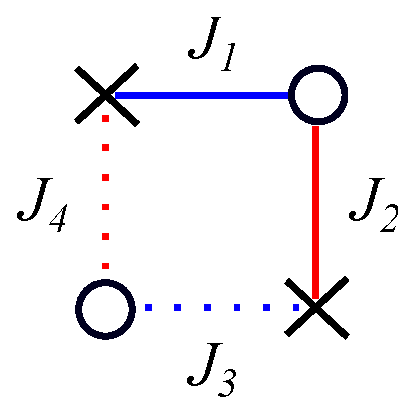
\includegraphics[width=0.7\linewidth]{Pictures/cell1.eps} \\ а)}
	\end{minipage}
	\hfill
	\begin{minipage}[h]{0.4\linewidth}
		\center{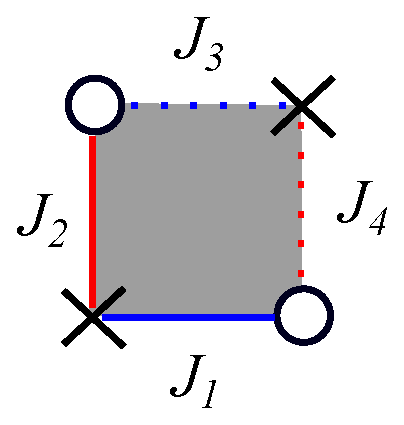
\includegraphics[width=0.7\linewidth]{Pictures/cell2.eps} \\ б)}
	\end{minipage}
	\caption{Два вида ячеек на обобщенной квадратной решетке}
	\label{cell}
\end{figure}

Возвращаясь к рассматриваемой работе, следует отметить, что обобщенная квадратная решетка с двумя трансляциями по горизонтали и вертикали, совпадает с так называемой «шахматной решеткой». Это легко увидеть, если оставить один тип ячеек обобщенной квадратной решетки (см. рис.\ref{gen}) незакрашенными (рис.\ref{cell}а), а другой — закрашенными (рис.\ref{cell}б). В результате получится решетка, показанная на рисунке~\ref{chessLattice}.

Фактически, Кастелайн и другие исследователи в своих работах рассматривали именно шахматную решетку. При этом каждый димер в решетке покрывает пару соседних узлов разных типов — в данной работе эти два типа узлов обозначены символами кружка ($\circ$) и креста ($\times$) (см. рис.~\ref{point}). Аналогично, при замощении квадратной решетки плитками домино каждая плитка покрывает две соседние, но различные ячейки, изображенные на рисунке~\ref{cell}.

\begin{figure}[h]
	\center{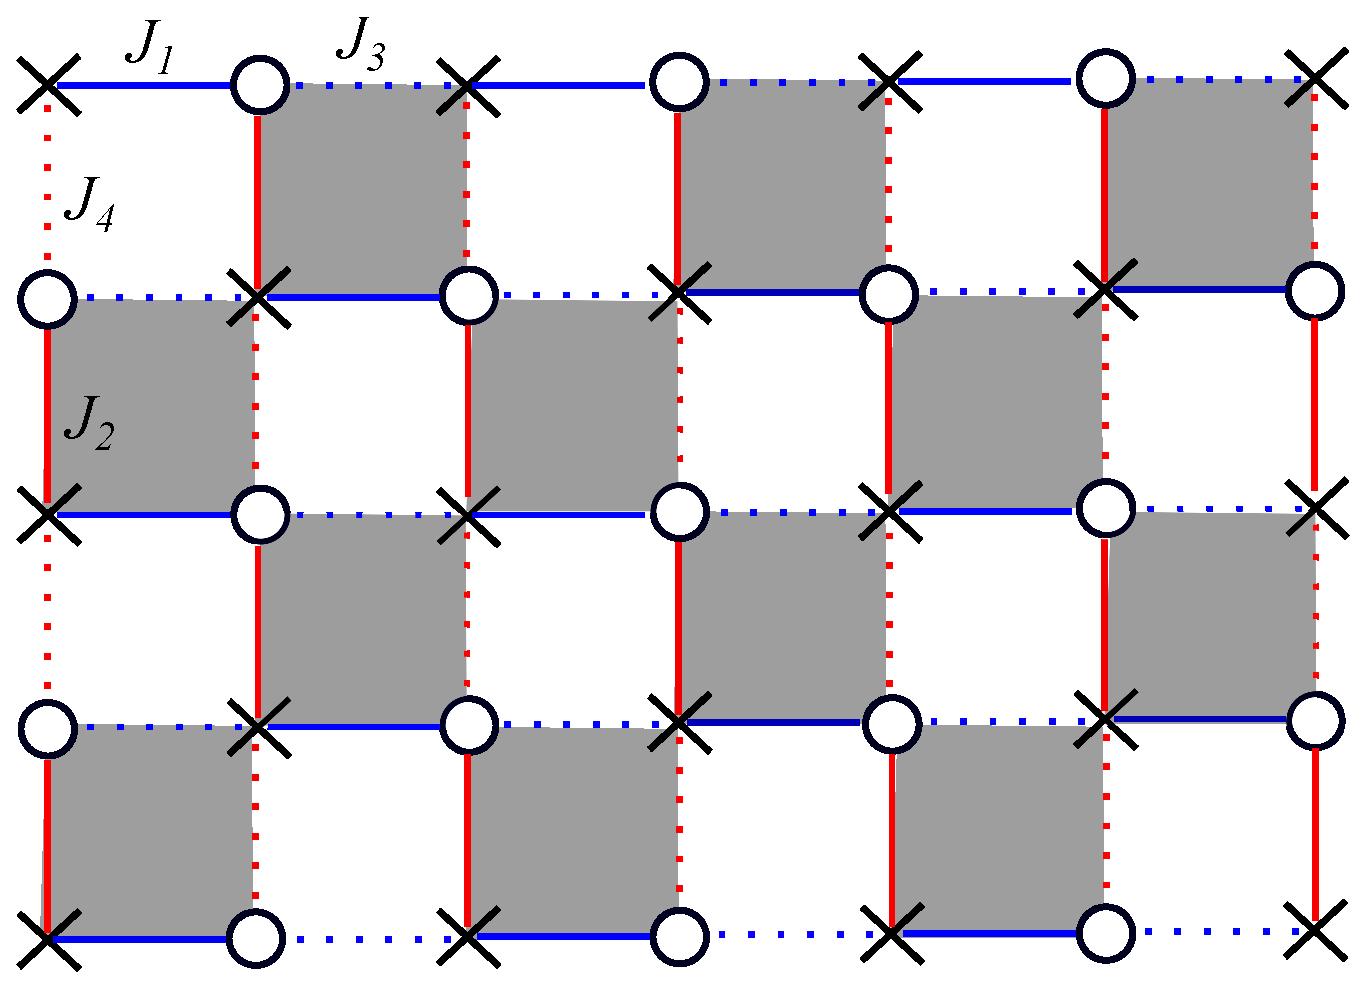
\includegraphics[width=0.5\linewidth]{Pictures/chessLattice.eps}}
	\caption{Шахматная решетка}
	\label{chessLattice}
\end{figure}

В рамках проведенного исследования получено значение нуль-температурной энтропии на один спин обобщенной квадратной решетки с двумя трансляциями, равное $G/\pi$. Кроме того, обнаружено еще одно значение нуль-температурной энтропии, равное $1/(2\pi)\Cl_2(\pi/3)$, что ровно в два раза меньше, чем значение нуль-температурной энтропии, найденное Ваннье для треугольной решетки~\cite{wannier1950}, равное $\Cl_2(\pi/3)/\pi = 0.3230\dots$.

Все эти факты свидетельствуют о глубокой связи между значениями фрустрационной энтропии в модели Изинга и комбинаторными задачами, такими как димерные покрытия и замощения плитками домино. Однако, данный тезис требует дальнейшей проверки и более тщательного теоретического обоснования.

\section{Заключение}
		
Таким образом, в настоящей работе впервые выведено точное аналитическое решение обобщенной модели Изинга с двумя трансляциями в горизонтальном и вертикальном направлениях на квадратной решетке комбинаторным методом Вдовиченко-Фейнмана. 

Анализ физических характеристик модели показал богатую картину поведения, включающую как классические случаи без фрустраций, так и разнообразные фрустрированные состояния с остаточной энтропией при нулевой температуре. Важным результатом является выявление двух фундаментальных значений нуль-температурной энтропии в антиферромагнетике, связанных со специальными математическими константами — постоянной Каталана и функцией Клаузена, а также выражения для свободной энергии Гельмгольца в ферромагнетике в точке фазового перехода, также связанного с постоянной Каталана. Эти значения отражают глубокую связь фрустраций в модели Изинга с комбинаторными задачами, такими как замощение решетки плитками домино.

Кроме того, исследование продемонстрировало, что при варьировании знаков и величин обменных взаимодействий можно наблюдать новое свойство фрустрированных спиновых систем, а именно, появление дополнительного пика теплоемкости, причину которого еще предстоит выяснить. Также, варьирование знаков и величин обменных взаимодействий позволяет трансформировать структуру обобщенной решетки, вплоть до перехода к топологически различным решеткам (например, к треугольной или искаженной решетке Кагоме). Это подчеркивает универсальность и гибкость обобщенной модели Изинга для описания широкого спектра магнитных и фрустрированных систем.

Наконец, установлена тесная связь между фрустрационной энтропией обобщенной модели Изинга и классической задачей подсчета димерных покрытий (замощений плитками домино), что открывает перспективы для дальнейших исследований, объединяющих методы статистической физики, комбинаторики и теории графов. 

В заключении данной работы следует сказать, что обобщенная модель Изинга позволяет исследовать и изучать как целое многообразие новых еще неизведанных решеток, так и решетки, которые давно известны, но до сих приковывают взгляды ученых по всему миру.
		
%Работа выполнена в рамках государственного задания Министерства науки и высшего образования РФ (тема «Квант», No АААА-А18-118020190095-4) при частичной поддержке Уральского отделения Российской академии наук (проект No 18-2-2-11).
	
%========================================================================
	
\begin{references}

\bibitem{ising1925} E.~Ising, Zeitschrift für Physik \textbf{21}, 253 (1925).
\bibitem{peierls1936} R.~Peierls, Proc. Cambridge Phil. Soc., \textbf{32}, 477 (1936).
\bibitem{kramers_wannier1}  H.A.~Kramers, G.H.~Wannier, Phys. Rev. \textbf{60}, 252 (1941).
\bibitem{kramers_wannier2}  H.A.~Kramers, G.H.~Wannier, Phys. Rev. \textbf{60}, 263 (1941).
\bibitem{onsager1941}  L.~Onsager, Phys. Rev. \textbf{65}, 117 (1944).
\bibitem{kac1952} M.~Kac, J.C.~Ward, Phys. Rev. \textbf{88}, 1332 (1952).
\bibitem{potts1955} R.B.~Potts, J.C.~Ward, Prog. Theor. Phys. \textbf{13}, 38 (1955).
\bibitem{hurst1960} C.A.~Hurst, H.S.~Green, J. Chem. Phys. \textbf{33}, 1059 (1960).
\bibitem{vdovichenko1964} N.V.~Vdovichenko, ЖЭТФ \textbf{47}, 715 (1964).
\bibitem{vdovichenko1965} N.V.~Vdovichenko, ЖЭТФ \textbf{48}, 526 (1965).
\bibitem{feynman1972} R.P.~Feynman, Statistical Mechanics. A Set of Lectures. Addison-Wesley, Reading, MA, (1972).
\bibitem{samuel1980} S.~Samuel, J. Math. Phys. \textbf{21}, 2015 (1980).
\bibitem{plechko1985} В.Н.~Плечко, ТМФ, \textbf{64}, 150 (1985).
\bibitem{vergeles2009} С.Н.~Вергелес, ЖЭТФ \textbf{135}, 820 (2009).
\bibitem{grunbaum1987} B.~Grünbaum, G.C.~Shephard, Tilings and Patterns, Freeman, New York, (1987).
\bibitem{wannier1950}  G.H.~Wannier, Phys. Rev. \textbf{79}, 357 (1950).
\bibitem{houtapell1950} R.M.F.~Houtappel, Prog. Theor. Phys. \textbf{16}, 425 (1950).
\bibitem{kano_naya1953}  K.~Kanô, S.~Naya, Prog. Theor. Phys. \textbf{10}, 158 (1953).
\bibitem{lin1983} K.Y.~Lin, W.J.~Ma, J. Phys. A: Math. Gen. \textbf{16}, 3895, (1983).
\bibitem{lin1985} K.Y.~Lin, W.N.~Huang, Aust. J. Phys., \textbf{38}, 227, (1985).
\bibitem{vaks1965} В.Г.~Вакс, А.И.~Ларкин и Ю.Н.~Овчинников, ЖЭТФ, \textbf{49}, 1180 (1965).
\bibitem{urumov2002} V.~Urumov, J. Phys. A: Math. Gen. \textbf{35}, 7317, (2002).
\bibitem{holzer1990} M.~Holzer, Phys. Rev. B \textbf{42}, no.16, 10570, (1990).
\bibitem{lin1988} K.Y.~Lin and S.C.~Wang, Phys. Letters A, \textbf{128}, (1988).
\bibitem{oitmaa2002} J.~Oitmaa and M.~Keppert, J. Phys. A: Math. Gen. \textbf{35}, L219 (2002).
\bibitem{strecka2008} J.~Strečka, L.~Čanová, Acta Phys. Pol. A \textbf{113}, 457 (2008). 
\bibitem{chao1990} N.C.~Chao, F.J.~Lee and K.Y.~Lin, Int. Journal of Modern Physics B \textbf{4}, No.1, 113 (1990).
\bibitem{loh2008} Y.L.~Loh, D.X.~Yao, and E.W.~Carlson, Phys. Rev. B \textbf{77}, 134402 (2008).
\bibitem{chikyu1987} T.~Chikyu, M.~Suzuki, Prog. Theor. Phys. \textbf{78}, (6), 1242 (1987).
\bibitem{morita1986} T.~Morita, J. Phys. A: Math. Gen. \textbf{19}, 1701 (1986).
\bibitem{wu1987} F.Y.~Wu, K.Y.~Lin, J. Phys. A: Math. Gen. \textbf{20}, 5737 (1987).
\bibitem{syozi1972} I.~Syozi, Transformation of Ising models, in Phase transitions and Critical Phenomena Vol. 1. Exact Results, edited by C.~Domb and M.S.~Green (Academic Press, London, 1972), pp. 270–329.
\bibitem{utiyama1951} T.~Utiyama, Prog. Theor. Phys. \textbf{6}, 907 (1951).
\bibitem{warden1941} B.L.~van der Waerden, Z. Physik \textbf{118}, 473 (1941).
\bibitem{kaufman1949} B.~Kaufman and L.~Onsager, Phys. Rev. \textbf{76}, 1244, (1949).
\bibitem{generalizedIsing2021} Е.С.~Цуварев, Ф.А.~Кассан-Оглы, ЖЭТФ \textbf{160}, 232 (2021).
\bibitem{mussardo2010}  G.~Mussardo, Statistical field theory: An introduction to exactly solved models in statistical physics (Oxford Graduate Texts), New York: Oxford University Press Inc., (2010).
\bibitem{abramowitz_stegun1972} M.~Abramowitz, A.~Stegun, Handbook of mathematical functions with formulas, graphs, and mathematical tables, Applied Mathematics Series, Washington D.C.; New York: United States Department of Commerce, National Bureau of Standards; Dover Publications (1972).
\bibitem{wood1968} Van E.~Wood, Math. Comp. \textbf{22}, 883 (1968).
\bibitem{kasteleyn1961} P.W.~Kasteleyn, Physica \textbf{27}, 1209 (1961).
\bibitem{kasteleyn1963_1} P.W.~Kasteleyn, J. Math. Phys. \textbf{4}, 287 (1963).
\bibitem{kasteleyn1963_2} P.W.~Kasteleyn, Physica \textbf{29}, 1329 (1963).
\bibitem{temperley1961} H.N.V.~Temperley, M.E.~Fisher, Philosophical Magazine \textbf{6}, 1061 (1961).
\bibitem{fisher1966} M.E.~Fisher, J. Math. Phys. \textbf{7}, 1776 (1966).
\end{references}
	
\end{document}






